\documentclass[a4paper,12pt]{article}
\usepackage[swedish]{babel}
\usepackage[utf8]{inputenc}
\usepackage{graphicx}
\usepackage[title]{appendix}
\usepackage{amsmath}
\usepackage{epstopdf}
\usepackage{pdfpages}
\usepackage{xparse}
\usepackage{kantlipsum}
\usepackage{listings}
\usepackage{subcaption}
\usepackage{float}
\usepackage{titlesec}
\usepackage{subcaption}
\usepackage[utf8]{inputenc}
\usepackage[T1]{fontenc}
\usepackage{times}
\usepackage{ifthen}
\usepackage[margin=25mm]{geometry}
\usepackage{fancyhdr}
\pagestyle{fancy}
\setlength{\parindent}{0pt}
\setlength{\parskip}{1ex plus 0.5ex minus 0.2ex}
\newcommand{\twodigit}[1]{\ifthenelse{#1<10}{0}{}{#1}}
\newcommand{\dagensdatum}{\number\year-\twodigit{\number\month}-\twodigit{\number\day}}

%% ------------------------------------------
% NYBILD
% Skapar centrerad bild med caption
%
% #1: Filens url relativt '/images/'
% #2: Caption
% #3: Label
% #4: Skalning
%% ------------------------------------------
\newcommand{\nyBild}[4]{
    \begin{figure}[H]
        \centering
        \includegraphics[angle=0,scale=#4]{images/#1}
        \caption{#2}
        \label{fig:#3}
    \end{figure}
}

%%  Redefinitions of commands containing @
\makeatletter
\makeatother

\newcommand{\LIPStitelsida}{
    {\ }\vspace{45mm}
    \begin{center}
        \textbf{\Huge \LIPSdokumenttyp}
    \end{center}
    \begin{center}
        {\large Alexander Vevstad, Amanda Aasa, Amanda Svennblad, \\Daniel Thomas, Lina Larsson, Olav Berg}
    \end{center}
    \begin{center}
        {\large \textbf{Version \LIPSversion}}
    \end{center}
    \begin{center}
        {Parts of chapter \ref{ch:intro} and \ref{ch:install} are based on the 2019 user guide for ENVISIoN.}
    \end{center}
    \vfill
    \begin{center}{
        \large Status}\\[1.5ex]
        \begin{tabular}{|*{3}{p{40mm}|}}
            \hline
            Granskad & \LIPSgranskare & \LIPSgranskatdatum \\
            \hline
            Godkänd & \LIPSgodkannare & \LIPSgodkantdatum \\
            \hline
        \end{tabular}
    \end{center}
}


\newenvironment{LIPSdokumenthistorik}{
    \begin{center}
        Document history\\[1ex]
        \begin{small}
            \begin{tabular}{|l|l|p{60mm}|l|l|}
                \hline
                \textbf{Version} & \textbf{Date} & \textbf{Changes} &
                \textbf{Done by} & \textbf{Reviewed} \\
                }
                {
                \hline
            \end{tabular}
        \end{small}
    \end{center}
}


\newcommand{\LIPSversionsinfo}[5]{\hline {#1} & {#2} & {#3} & {#4} & {#5} \\}
\newcounter{LIPSkravnummer}
\newcounter{LIPSunderkravnummer}[LIPSkravnummer]

\newenvironment{LIPSkravlista}{
    \begin{tabular}{|p{25mm}|p{25mm}|p{85mm}|p{5mm}|}
        }
        {
        \hline
    \end{tabular}
}

\newenvironment{LIPSleveranslista}{
    \begin{tabular}{|p{25mm}|p{15mm}|p{70mm}|p{25mm}|p{5mm}|}
        }
        {
        \hline
    \end{tabular}
}

\newenvironment{tabellexlista}{
    \begin{tabular}{|p{25mm}|p{25mm}|p{70mm}|p{20mm}|}
        }
        {
        \hline
    \end{tabular}
}

\newenvironment{dokumentlista}{
    \begin{tabular}{|p{28mm}|p{17mm}|p{39mm}|p{28mm}|p{28mm}|}
        }
        {
        \hline
    \end{tabular}
}

\newcommand{\dokumenttext}[5]{
    \hline 
    {#1} & {#2} & {#3} & {#4} & {#5} \\
}


\newcommand{\LIPSkrav}[3]{
    \hline
    \stepcounter{LIPSkravnummer}
    \textbf{Krav nr \arabic{LIPSkravnummer}} & \textbf{{#1}} & {#2} & \textbf{{#3}} \\
}

\newcommand{\tabellex}[3]{
    \hline
    Krav nr x & {#1} & {#2} & {#3} \\
}

\newcommand{\LIPSleverans}[2]{
  {#1} & {#2} & \hline
}

\newcommand{\LIPSunderkrav}[3]{
    \hline\stepcounter{LIPSunderkravnummer}\textbf{Krav nr \arabic{LIPSkravnummer}\Alph{LIPSunderkravnummer}} & \textbf{{#1}} & {#2} & \textbf{{#3}} \\
}

\newenvironment{LIPSprojektidentitet}{%
{\ }\vspace{45mm}
\begin{center}
  {\Large PROJECT IDENTITY}\\[0.5ex]
  {\small
  \LIPSartaltermin, \LIPSprojektgrupp\\
  Faculty of Science and Engineering, Linköping University, IFM
  }
\end{center}
\begin{center}
  {\small Group members}\\
%  \begin{tabular}{|p{30mm}|p{40mm}|p{35mm}|p{45mm}|}
  \begin{tabular}{|l|p{45mm}|p{25mm}|l|}
    \hline
    \textbf{Name} & \textbf{Role} & \textbf{Phone nr.} & \textbf{E-mail} \\
    \hline
}%
{%
    \hline
  \end{tabular}
\end{center}
\begin{center}
  {\small
    \textbf{Website}: \LIPSgrupphemsida\\[1ex]
    \textbf{Client}: \LIPSkund\\
    \textbf{Contact person of client}: \LIPSkundkontakt\\
    \textbf{Course examintor}: \LIPSkursansvarig\\
    \textbf{Main supervisor}: \LIPShandledare\\
  }
\end{center}
\newpage
}
\newcommand{\LIPSgruppmedlem}[4]{\hline {#1} & {#2} & {#3} & {#4} \\}

\NewDocumentCommand\secpdf{somO{1}m}{
  \clearpage
  \thispagestyle{fancy}
  \addcontentsline{toc}{section}{#3}
  \includepdf[
    pages=#4,
    pagecommand={
      \IfBooleanTF{#1}{
        \section*{#3}}{
        \IfNoValueTF{#2}{
          \section{#3}}{
          \section[#2]{#3}}}},
    scale=.80
    ]
    {#5}
}

\newenvironment{LIPSlicens}{
    \begin{center}
    \large{Licens}
    \end{center}
}{}

\graphicspath{ {./images/} }
\lstset{literate=%
{å}{{\aa}}1
{ä}{{\"a}}1
{ö}{{\"o}}1
{Å}{{\AA}}1
{Ä}{{\"A}}1
{Ö}{{\"O}}1
}

\newcommand{\LIPSartaltermin}{2019/VT}
\newcommand{\LIPSkursnamn}{TFYA75}

\newcommand{\LIPSprojekttitel}{Elektronvisualisering}
\newcommand{\LIPSdokumenttyp}{Teknisk dokumentation}
\newcommand{\LIPSversion}{1.0}
\newcommand{\LIPSdatum}{\dagensdatum}

\newcommand{\LIPSgranskare}{}
\newcommand{\LIPSgranskatdatum}{}
\newcommand{\LIPSgodkannare}{}
\newcommand{\LIPSgodkantdatum}{}

\lhead{}
\chead{\textbf{\LIPSprojekttitel}}
\rhead{\textbf{\textsl{LiTH}}\\\textbf{\dagensdatum}}
\lfoot{\textbf{LIPS Teknisk dokumentation}}
\cfoot{\textbf{\thepage}}
\rfoot{\textbf{\LIPSkursnamn}}

\begin{document}
\pagenumbering{gobble}
\LIPStitelsida
\newpage
\pagenumbering{roman}
\newcommand{\LIPSgruppepost}{finns ej}
\newcommand{\LIPSgrupphemsida}{https://liuonline.sharepoint.com/sites/TFYA75/TFYA75\_2019VT\_7Z/62340}

\newcommand{\LIPSdokumentansvarig}{Abdullatif Ismail}
\newcommand{\LIPSkund}{Rickard Armiento, IFM, Linköpings universitet, 581\ 83 Linköping}
\newcommand{\LIPSkundkontakt}{Rickard Armiento, rickard.armiento@liu.se}
\newcommand{\LIPSkursansvarig}{Per Sandström, per.sandstrom@liu.se}
\newcommand{\LIPShandledare}{Johan Jönsson, johan.jonsson@liu.se}

%% Argument till \LIPSgruppmedlem: namn, roll i gruppen, telefonnummer, epost
\begin{LIPSprojektidentitet}
  \LIPSgruppmedlem{Linda Le}{Projektledare (PL)}{076-2249926}{linle336@student.liu.se}
  \LIPSgruppmedlem{\LIPSdokumentansvarig}{Dokumentansvarig (DOK)}{072-0355455}{abdis077@student.liu.se}
  \LIPSgruppmedlem{Anton Hjert}{Anton Hjert (AH)}{070-5728891}{anthj975@student.liu.se}
  \LIPSgruppmedlem{Jesper Ericsson}{Jesper Ericsson (JE)}{070-8772630}{jeser991@student.liu.se}
  \LIPSgruppmedlem{Lloyd Kizito}{Lloyd Kizito (LK)}{070-8230589}{lloki004@student.liu.se}
\end{LIPSprojektidentitet}
\newpage
\tableofcontents{}
\newpage
%% Argument till \LIPSversionsinfo: versionsnummer, datum, ändringar, utfört av, granskat av
\addcontentsline{toc}{section}{Dokumenthistorik}
\begin{LIPSdokumenthistorik}
  \LIPSversionsinfo{0.1}{2019-05-21}{Första utkast.}{Projektgruppen}{Projektgruppen}
  \LIPSversionsinfo{1.0}{2019-05-25}{Andra utkast. Kompletterade enligt kommentarer från beställare.}{Projektgruppen}{Projektgruppen}
\end{LIPSdokumenthistorik}
\newpage
\addcontentsline{toc}{section}{Licens}
\begin{LIPSlicens}
    2019 års modifikationer av den tekniska dokumentationen är licensierade under BSD, se bilaga~\ref{ref:licens}. 
\end{LIPSlicens}

\newpage
\pagenumbering{arabic}
\section{Inledning}
Elektronstrukturberäkningar är ett viktigt verktyg inom teoretisk fysik för att förstå hur materials och molekylers egenskaper kan härledas från kvantmekaniska effekter. För att förstå dessa egenskaper är det viktigt att kunna analysera data från beräkningarna, något som förenklas och görs möjligt genom visualisering. ENVISIoN är en kraftfull mjukvara som är avsedd för visualisering av data från beräkningsprogram som VASP. Mjukvaran bygger på forskningsverktyget Inviwo, utvecklad av Visualiseringscenter i Norrköping. Idén med ENVISIoN är att underlätta visualiseringarna från kvantmekaniska beräkningar. Det ska vara enkelt och smidigt att visualisera önskade och relevanta egenskaper hos olika system bestående av atomer. Mjukvaran tillgängliggör olika reglage och knappar för att på ett interaktivt sätt kunna ändra dess egenskaper. I följande dokument kommer de tekniska aspekterna av hur systemet är implementerat att redovisas.  

\subsection{Parter}
ENVISIoN är en produkt som beställts av beställaren Rickard Armiento. Produkten har skapats av projektgruppen, redovisade under projektidentiteten, under handledning av handledare Johan Jönsson. Se projektidentitet för mer genomgående information om beställare och handledare.    

%Beställare: \LIPSkund \\
%Leverantör: Grupp 1.

\subsection{Projektets bakgrund} 
%Visualisering och simulering av beräkningsresultat är mycket väsentligt för förståelsen hos olika sorterts analyser. Syftet med ENVISIoN är att visualisera kvantmekaniska beräkningar för att underlätta analyseringen av resultaten. När mjukvaran är klar är syftet att den används i forskningssyften. 
Projektet skapades i samband med kandidatarbetet, kursen TFYA75. Som ett väsentligt examinerade moment ska projektet genomförande återspegla alla förutsättningar, krav och ansvarstaganden som råder under en formell anställning. Utveckling av ENVISIoN är en av flera projekt som kan väljas inom kursen. Produktens slutgiltiga syfte är att användas som ett forskningsverktyg for visualisering av kvantmekaniska beräkningar.      

\subsection{Syfte och mål}
Projektet syftar till att utveckla kreativiteten samt att ge färdigheter i fysikalisk tänkande och analys av teoretiska resultat. Projektet bedrivs realistiskt som en träning inför det kommande yrkeslivet. Resultatet av projektarbetet ska hålla hög vetenskaplig och teknisk kvalité och baseras på moderna kunskaper, dokumenteras i form av projekt-och tidsplan, krav-och designspecification samt i en teknisk/vetenskaplig rapport, presenteras muntligt, demonstreras och följas upp i en efterstudie. Målet är att i visualiseringsverktyget Inviwo utveckla ett system för visualisering av resultatet av elektronstrukturberäkningar. Att demonstrera systemetsfunktionalitet genom att använda det till att illustrera några befintliga beräkningsresultat.

\subsection{Användning}
Denna produkt kommer huvudsakligen användas vid Linköpings universitet för att analysera data från elektronstruktursberäkningar.

\subsection{Begränsningar}
I projektet kommer visualiseringsverktyget Inviwo och programmeringspråken Python och C++ användas. Det kommer inte utredas om det är bättre att använda andra verktyg.

\subsection{Definitioner}
\begin{itemize}
\setlength\itemsep{0em}
\item \textbf{Inviwo:} Ett forskningsverktyg som utvecklas vid Linköpings universitet och ger användaren möjlighet att styra visualisering med hjälp av programmering i Python3 eller grafiskt. Det tillhandahåller även användargränssnitt för interaktiv visualisering. \cite{Inviwo}

\item \textbf{Processor:} Benämningen på ett funktionsblock i Inviwos nätverksredigerare som tar emot indata och producerar utdata. I detta dokument avser en processor alltid en inviwoprocessor om inte annat anges.

\item \textbf{Canvas:} En processor i Inviwo som ritar upp en bild i ett fönster.

\item \textbf{Data frame:} En tabell med lagrad data i form av tal. Varje kolumn i tabellen har ett specifikt namn.

\item \textbf{Transferfunktion:} Begrepp inom volymrendering för den funktion som används för att översätta volymdensiteter till en färg.

\item \textbf{Transferfunktionspunkt: } Ett värde i transferfunktionen som definerar en färg vid ett speciellt densitetsvärde.

\item \textbf{Port:} Kanal som processorer använder för att utbyta data av specifika typer.

\item \textbf{Property:} En inställning i en Inviwoprocessor.

\item \textbf{Länkar:} Kanaler som processorer använder för att länka samman properties av samma typ så att deras tillstånd synkroniseras.

\item \textbf{Nätverk:} Ett antal processorer sammankopplade via portar och länkar. 

\item \textbf{Volymdata:} Tredimensionell data som beskriver en volym.

\item \textbf{API:} Application Programming Interface, en specifikation av hur olika applikationer kan användas och kommunicera med en specifik programvara. Detta utgörs oftast av ett dynamiskt länkat bibliotek.\cite{API}

\item \textbf{BSD2:} En licens för öppen källkod.
	\cite{BSD2}

\item \textbf{C++:} Ett programmeringsspråk.
	\cite{C++}
	\newline
	I Inviwo används C++ för att skriva programkod till processorer.

\item \textbf{Python3:} Ett programmeringsspråk.
	\cite{Python3}
	\newline
	I Inviwo används Python3 för att knyta samman processorer.

\item \textbf{Fermienergi:} Energinivån där antalet tillstånd som har en energi lägre än Fermienergin är lika med antalet elektroner i systemet. \cite{Fermi-energi}

\item \textbf{Git:} Ett decentraliserat versionshanteringssystem.
\cite{Git}
    
\item \textbf{GUI:} (Graphical User Interface) Ett grafiskt
användargränssnitt.
\cite{GUI}

\item \textbf{PyQT:} En python-modul för GUI-programmering.\cite{PyQT}

\item \textbf{wxPython:} En samling av python-moduler för GUI-programmering.\cite{wxPython}

\item \textbf{PKF} En förkortning på Parkorrelationsfunktionen. Vilket ibland slarvigt kan anges synonymt som RDF, Radial Distribution Function.

\item \textbf{HDF5:} Ett filformat som kan hantera stora mängder data. Alla HDF5-objekt har en rotgrupp som äger alla andra objekt i datastrukturen. Denna grupp innehåller i sin tur all övrig data i form av andra grupper, länkar till andra grupper eller dataset. Dataset innehåller rådata av något slag. Rådata kan i sammanhanget vara bilder, utdata från beräkningar, programdata, etc. \cite{HDF group} \cite{HDF group2} 

De övriga objektstyperna gås inte igenom i detalj i detta dokument,
men finns väl beskrivna i \emph{High Level Introduction to HDF5} \cite{HDF group2}.

%\item \textbf{Metadata} - Data som beskriver rådatan i HDF5 filstrukturen. 
\item \textbf{VASP:} The Vienna Ab initio simulation package, ett program för modellering på atomnivå, för t.ex. elektronstruktusrberäkningar och kvantmekanisk molekyldynamik.
\cite{VASP}

\item \textbf{Parser:} Ett system som översätter en viss typ av filer till en annan typ av filer. I detta fall sker översättningen från textfiler, genererat i beräkningsprogrammet VASP, till HDF5-filer.

\item \textbf{Parsning:} Översättning utförd av parsern.

\item \textbf{Mesh} - Beskriver ett geometriskt objekt som en uppsättning av ändliga element. 

\item \textbf{array} - Ett dataobjekt som fungerar som behållare för element av samma typ \cite{what is array}.  

\item \textbf{UNIX} - Benämning av en grupp operativsystem som härstammar från UNIX System from Bell Labs \cite{what is UNIX}.   
\end{itemize}


\newpage
\newpage
\section{Översikt av systemet}
\nyBild{oversikt.png}{Enkel skiss över ENVISIoN systemet}{oversikt}{0.8}

Den produkt som utvecklas är ett verktyg för att visualisera viktiga egenskaper från elektronstrukturberäkningar. Systemet skall bestå av ett användargränssnitt där användaren får välja vilka beräkningsresultat som skall konverteras och visualiseras.

I figur \ref{fig:oversikt} visas en grov systemskiss med de olika delsystem som ingår. Systemet kan grovt delas upp i tre olika delar. Ett system för parsning av datafiler från exempelvis VASP, ett system för att visualisera det som parsas i tidigare nämnt system, och ett GUI-system vilket användaren interagerar med visualiseringen via.

\subsection{Ingående delsystem}
Systemet för elektronvisualisering består i huvudsak av tre delar. Dels består systemet av en parsing-del där textfiler genererade från beräkningsprogrammet VASP skall översättas till det, med vår mjukvara, kompatibla filformatet HDF5. 

När denna filkonvertering är klar så ska de genererade filerna behandlas i ett visualiseringssystem för att skapa önskade visualiseringar. Visualiseringen i Inviwo byggs upp av processorer vilka datan låts flöda igenom för att skapa önskat slutresultat.

Den sista delen av systemet är det som möter användaren, det grafiska användargränssnittet, GUI:t.
Genom detta system skall tillgång till att starta och göra ändringar i visualiseringen ges. Målet är att kunna styra hela systemet från GUI:t som en fristående del från de två första delsystemen.
\newpage
\section{Parsersystemet} 
Parserystemets uppgift är att omvandla information från VASP-filer till data i HDF5-format, som visualiseringssystemet kan använda. Parsersystemet är det delsystem i ENVISIoN som ser till att avläsa korrekt data från VASP-filer och spara denna data i en lämplig HDF5-filstruktur. Följande kapitel beskriver hur parsersystmet har implementerats, samt redogör bakgrundskunskaper om HDF5 och VASP.  

\subsection{Bakgrundskunskap}
För förståelse över hur parsersystemet implementerats krävs det lite bakgrundskunskaper om hur HDF5 är uppbyggt och vad VASP är.   
\subsubsection{VASP}
VASP är ett beräkningsprogam som använder sig av Hartree-Fock metoden eller täthetsfunktionalteori (DFT) för att approximera en lösning för Schrödingerekvationen för mångpartikelfallet \cite{Quick Start Guide}. VASP-filer kan delas upp i indatafiler och utdatafiler. I indatafiler anges information som användaren kan manipulera, dessa indatafiler styr hur beräkningarna ska utföras. Efter beräkningar genereras sedan ett antal utdatafiler som innehåller kalkylresultaterna. Varje datafil korresponderar till specifik information om systemet. Nedan återfinns några viktiga VASP-filer.   

\textbf{Utdatafiler:} 
\begin{itemize}
    \setlength\itemsep{0em}
    \item CHG innehåller data om laddningstäthet.
    \item DOSCAR innehåller data om tillståndstäthet.
    \item EIGENVAL innehåller data för alla energier för k-rummet.
    \item OUTCAR innehåller alla utdata.   
    \item XDATCAR innehåller data om enhetscell, atompositioner för varje beräkningssteg och även atomstyp. 
    \item CONTCAR innehåller data som den återfunnen i POSCAR, men innehåller information om atompositioner uppdateras.  
    \item PCDAT Innehåller data för parkorrelationsfunktionen, PKF.  
\end{itemize}

\textbf{Indatafiler:} 
\begin{itemize}
    \setlength\itemsep{0em}
    \item INCAR innehåller information, i form av flaggor över hur beräkningar ska ske.
    \item POSCAR innehåller data om enhetcellen och atompositionering. 
    \item POTCAR innehåller data om atomtyper.
\end{itemize}

\newpage
Vid exempelvis beräkning av PKF för Si i temperaturen 300K, specificeras information om hur systemet ser ut i filer som POSCAR. Sedan kan information om hur beräkningarna ska genomföras specificeras i exempelvis INCAR eller POTCAR. Detta kan röra sig om hur många iterationer som ska ske och i vilka avstånd PKF ska beräknas. Då kan exempelvis flaggor som NPACO och APACO sättas i INCAR-filen. Där flaggan NPACO specificerar hur många iterationer som sker och APACO bestämmer det längsta avståndet som sista iteration ska ha.

Efter beräkningen genereras flera utdatafiler, däribland PCDAT, som innehåller värdena av PKF. Utdatafilen, PCDAT, kan då ha följande utseende:
\nyBild{PCDAT_utseende.pdf}{En demonstrativ bild över utseendet för PCDAT från VASP. Notera att värdena inte riktigt stämmer.}{PCDAT-utseende}{0.5}

Bilden \ref{fig:PCDAT-utseende} beskriver utseendet hos en del av PCDAT-filen för PKF för systemet Si i 300K, med 40 olika tidsteg. Viktigaste är den långa kolumnen av siffror som utgör definitionsmängden till funktionen. 

\subsubsection{HDF5-format} \label{sssec:rotgruppstr}
Vid hantering av stora mängder data, sådana genererade av beräkningsprogram som VASP, är HDF5-formatet mycket användbart. Det gör specificiering av olika dataförhållanden och beroenden enkla, samt tillgängliggör bearbetning av delar av data åt gången.   

En HDF5-fil är ett objekt som innehåller en rotgrupp, som äger alla andra grupper under den. Denna rotgrupp kan symboliseras av $"$\textit{/}$"$. Exempelvis $"$\textit{/foo/zoo}$"$ symboliserar \textit{zoo} som är en medlem till \textit{group} \textit{foo}, 
som vidare är en medlem till rotgruppen. 
Ett \textit{dataset} kan pekas av flera \textit{groups}. \cite{High Level Introduction to HDF5}

\nyBild{DemonstrativHDF5bild.png}{Schematisk bild över HDF5 struktur}{}{0.55}

Mer ingående består \textit{dataset}-objektet av metadata och rådata. Metadata beskriver rådatan, till den ingår \textit{dataspace}, \textit{datatype}, \textit{properties} och \textit{attributes}. Alla dessa är HDF5-objekt som beskriver olika saker. 

\textit{datatype} beskriver vad för datatyp varje individuell dataelement i ett dataset har. Exempelvis kan detta vara ett 32-bitars heltal, eller ett 32-bitars flyttal. I det mer komplexa fallet kan det också vara en sammansättning av flera, vanligt benämnda, datatyper. \textit{Datatype} beskriver då en följd av olika datatyper. Exempelvis en sammansättning som int16, char, int32, 2x3x2 array av 32-bit floats beskriver att varje dataelement i det gällande datasetet har en datatyp som består av 16 bitars heltal, en bokstav, 32-bitars heltal och slutligen en array av flyttal med dimensionen 2x3x2. \textit{dataspace} är en HDF5-objekt som beskriver hur datasetet sparar sin data, den kan exempelvis vara tom. Ett dataset kan även bestå av ett enda tal, eller vara en array. 
\newpage
\textit{Properties} är mindre konkret än de två tidigare nämnda egenskaperna och beskriver minneshanteringen av ett dataset. I dess defaultläge exempelvist är dataset sparade kontinuerligt. Slutligen återfinns HDF5-objektet \textit{attributes}, som kan valbart skapas. Typiskt sätt skapas \textit{attributes} som ett sätt för att ytterligare beskriva några egenskaper hos ett dataset. En \textit{attribute} innehåller ett namn och ett värde, och skapas i samband med att en dataset öppnas. \cite{HDF group2}       


\nyBild{Dataset_Metadata_HDF5.png}{Schematisk bild över \textit{dataset}.}{}{1}

ENVISIoN arbetar med HDF5-formatet. Python ger tillgång till hantering av HDF5-formatet via paketet \textit{h5py}. Detta tillgängliggör exempelvis läsandet av specifika element i massiva arrayer med användandet av syntaxer tillgängliga av paketet \textit{numpy}. \cite{How To Use HDF5 Files in Python}

Paketet \textit{h5py} ger upphov till HDF5-filer vilket kan ses som behållare för två sorters objekt, \textit{datasets} och \textit{groups}. \textit{datasets} är array-liknande ihopsättning av data, medan \textit{groups} fungerar som behållare för andra \textit{groups} eller \textit{datasets} \cite{How To Use HDF5 Files in Python}. Elementen i \textit{datasets} kan vara komplexa objekt. \textit{groups} kan återfinnas i andra \textit{groups}, detta ger därmed möjlighet till konstruktion av grupperingar av olika sammanhängande data. \textit{groups} och medlemmarna till \textit{groups} fungerar som mappar och filer i UNIX. Varje \textit{dataset} karaktäriseras exempelvis av en sökväg. \cite{High Level Introduction to HDF5}

\newpage
\subsection{ENVISIoNs HDF5-fil}
ENVISIoNs parsersystem använder sig av pythonmodulen \textit{h5py} för att generera en lämplig HDF5-filstruktur vid parsning. Den HDF5-strukturen som genereras återfinns i nedstående diagram. Notera att figuren visas som helbild i Appendix \ref{sec:appendixHDF5}.

\nyBild{UPDATE-hdf5-dataformat3modi.png}{En bild över HDF5-filstruktur som används i ENVISIoN.}{ENVISIoNsHDF5}{0.2}

I diagram \ref{fig:ENVISIoNsHDF5} nedan representeras olika grupper (\textit{groups}) av lådor med pilar (förutom lådorna vars brödtext är angiven i parantes), de sista lådorna i slutet av varje förgrening representerar olika \textit{dataset}. Diagrammet beskriver alltså hur information struktureras i en HDF5-fil som parsersystemet skapat. För att få tillgång till ett visst \textit{dataset} måste en sökväg anges. Denna sökväg är inget mer än en sträng bestående av olika grupper som beskriver hur ett \textit{dataset} nås från rotgruppen, se under rubrik \ref{sssec:rotgruppstr}. 

Varje \textit{dataset} kan bestå av ett antal olika fältnamn. Det fältnamn som alltid förekommer är \textit{value}, vilket beskriver den huvudsakliga datan som datasetet innehåller. Utöver det kan vissa andra fältnamn också förekomma, exempelvis "VariableName" vilket är olika attribut, \textit{attributes}, som beskriver andra egenskaper hos \textit{dataset} som kan vara intressant. 

Notera att diagram \ref{fig:ENVISIoNsHDF5} saknar viss information för DOS. DOS står för Density of States, översatt till tillståndstäthet. På grund av platsbrist har inte attributen skrivits ut för DOS. p-DOS, d-DOS(xy), Energy, grupper under DOS, med mera har attributen  

\begin{itemize}
 \item {\textbf{VariableName}} är fältets namn.
 \item{\textbf{VariableSymbol}} är en symbol som representerar variabeln. 
 \item{\textbf{QuantityName}} är ett för en människa läsligt namn på fältet. 
 \item{\textbf{QuantitySymbol}} är symbol som representerar storheten.
 \item{\textbf{Unit}} är storhetens fysikaliska enhet.
\end{itemize}

Notera också att \textit{float[x]} avser en lista med längd x, samt att alla grupper som är märkta med n är en metod att ange att det kan finns flera grupper på den nivån. Lådor vars rubrik är angivet inom parentes anger ett villkor för att den resterande sökvägen ska kunna skapas. Viktig anmärkning här är därför att dessa villkor inte ingår i HDF5-strukturen, de är inga grupper, och ingår därmed inte med sökvägen till de respektive dataseten. Under \textit{\/DOS} förekommer exempelvis en sådan låda med brödtexten \textit{(LORBIT=0)}, samt under förgreningen hos \textit{\/DOS\/Partial} förekommer en låda med angivelsen \textit{(ISPIN=0)}. Båda \textit{ISPIN} och \textit{LORBIT} är flaggor som kan sättas i INCAR-filen. I detta fall anger lådorna villkoren att \textit{(LORBIT=0)} och \textit{(ISPIN=0)} för att den fortsatta respektive grupperna under ska kunna skapas. Lådan under \textit{\/PairCorrelationFunc} anger dock ingen sådan flaggan. Det den anger är villkoret som har med huruvida \textit{\_write\_pcdat\_onecol} eller \textit{\_write\_pcdat\_multicol} används.

Parsning av PKF ges av olika möjligheter, parsern behandar en av följande fall: 

\begin{enumerate}
    \item System av flera atomtyper, det som beräknas är en genomsnittlig PKF över alla atomtyper.  
    \item System av flera atomtyper, det som beräknas är en genomsnittlig PKF för varje atomtyp. Ingår det K atomtyper i systemet ska parsern ge upphov till K stycken parkorrelationsfunktioner.
    \item System av 1 atomtyp. 
\end{enumerate}

För fall 2 och 3 används \textit{\_write\_pcdat\_multicol} medan fall 1 använder \textit{\_write\_pcdat\_onecol}, se under rubrik \ref{ssec:skrivning till HDF5}. Villkoren är därmed enbart ett sätt att ange vad för fall parsern behandlar. 
\newpage 

\subsection{Skrivning till HDF5-fil} \label{ssec:skrivning till HDF5}
Det som skapar strukturen i HDF5-filen är skrivningsmodulen \textit{h5writer} I ENVISIoN. \textit{h5writer.py} är ett skript som innehåller alla skrivningsfunktioner som ingår i parsersystemet. Funktionernas uppgift är att skapa \textit{datasets} (rådata) i rätt plats i HDF5-fil objektet. Nedan listas alla funktioner som ingår i modulen.

\textbf{\_write\_coordinates}
\newline 
Denna funktion skriver koordinater för atompositioner där varje atomslag tilldelas ett eget \textit{dataset}. Attribut sätts för respektive grundämnesbeteckning per \textit{dataset}.

Parametrar:
\begin{itemize}
    \setlength\itemsep{0em}
    \item h5file: Sökväg till HDF5-fil, anges som en sträng. 
    \item atom\_count: Lista med antalet atomer av de olika atomslagen.
    \item coordinates\_list: Lista med koordinater för samtliga atomer.     
    \item Elements: None eller lista med atomslag.      
\end{itemize}

Returnerar: 
\begin{itemize}
    \item None 
\end{itemize}

\textbf{\_write\_basis}
\newline 
Denna funktion skriver gittervektorerna i ett dataset med namn basis.

Parametrar:
\begin{itemize}
    \setlength\itemsep{0em}
    \item h5file: Sökväg till HDF5-fil, anges som en sträng.
    \item basis: Lista med basvektorerna.
\end{itemize}

Returnerar: 
\begin{itemize}
    \item None 
\end{itemize}

\textbf{\_write\_bandstruct}
\newline 
Denna funktion skriver ut data för bandstruktur i en grupp med namn Bandstructure. Inom denna grupp tilldelas specifika K-punkter, energier samt bandstrukturer egna dataset. Diverse attribut sätts även för bl.a. specifika energier.

Parametrar:
\begin{itemize}
    \setlength\itemsep{0em}
    \item h5file: Sökväg till HDF5-fil, anges som en sträng. 
    \item band\_data: Lista med bandstrukturdata.
    \item kval\_list: Lista med K-punkter för specifika bandstrukturdata.
\end{itemize}

Returnerar: 
\begin{itemize}
    \item None 
\end{itemize}

\textbf{\_write\_dos}
\newline 
Denna funktion skriver ut DOS-data i en grupp med namn DOS där total och partiell DOS tilldelas grupper med namn Total respektive Partial. Inom gruppen Total tilldelas energin samt specifika DOS egna dataset och inom gruppen Partial tilldelas varje partiell DOS egna grupper där energin samt specifika DOS tilldelas egna dataset.

Parametrar:
\begin{itemize}
    \setlength\itemsep{0em}
    \item h5file: Sökväg till HDF5-fil, anges som en sträng. 
    \item total: En lista med strängar av de olika uträkningarna som har utförts av VASP för total DOS.
    \item partial: En lista med strängar av de olika uträkningarna som har utförts av VASP för partiell DOS.
    \item total\_data: En lista med alla beräkningar för total DOS för varje specifik atom.
    \item partial\_list: En lista med alla beräkningar för partiell DOS för varje specifik atom.
    \item fermi\_energy: Fermi-energin för den aktuella uträkningen.
\end{itemize}

Returnerar: 
\begin{itemize}
    \item None 
\end{itemize}

\textbf{\_write\_volume}
\newline 
Denna funktion skriver ut elektrontäthetsdata och elektronlokaliseringsfunktionsdata (ELF) till grupper med namn CHG respektive ELF. Inom dessa grupper tilldelas varje iteration ett dataset.

Parametrar:
\begin{itemize}
    \setlength\itemsep{0em}
    \item h5file: Sökväg till HDF5-fil, anges som en sträng. 
    \item i: Skalär som anger numret på iterationen.
    \item partial:  En lista med strängar av de olika uträkningarna som har utförts av VASP för partiell DOS.
    \item array: Array med parsad data för respektive iteration.
    \item data\_dim: Lista som anger dimensionen av data för respektive iteration.
    \item hdfgroup: En textsträng med namnet på vad man vill kalla gruppen i HDF5-filen.
\end{itemize}

Returnerar: 
\begin{itemize}
    \item None 
\end{itemize}

\textbf{\_write\_incar}
\newline 
Denna funktion skriver ut parsad data från INCAR i ett dataset med namn Incar där varje datatyp tilldelas egna dataset.

Parametrar:
\begin{itemize}
    \setlength\itemsep{0em}
    \item h5file: Sökväg till HDF5-fil, anges som en sträng. 
    \item incar\_data: Datalexikon med all data från INCAR-filen.
\end{itemize}

Returnerar: 
\begin{itemize}
    \item None 
\end{itemize}

\textbf{\_write\_pcdat\_onecol}
\newline 
Denna funktion skapar ett HDF5-struktur för ett system med flera atomtyper, där en genomsnittlig PKF beräknas för alla atomtyper. Funktionen skapar en HDF5-struktur som innehåller data från huvudsakligen PCDAT. 

Parametrar:
\begin{itemize}
    \setlength\itemsep{0em}
    \item h5file: Sökväg till HDF5-fil, anges som en sträng. 
    \item pcdat\_data: Tillhör Python-datatypen \textit{dictionary} \cite{dict}. Detta argument innehåller alla värden av PKF som parsats.  
    \item APACO\_val: Värdet på APACO-flaggan i VASP-filen INCAR eller POTCAR. Defaultvärde är 16 Ångström. Flaggan anger det längsta avståndet sista iteration för beräkning av PKF har.     
    \item NPACO\_val: Värdet på NPACO-flaggan i VASP-filen INCAR eller POTCAR. Defaultvärde är 256. Flaggan anger hur många iterationer ska ske för beräkning av PKF.      
\end{itemize}

Returnerar: 
\begin{itemize}
    \item None 
\end{itemize}

\textbf{\_write\_pcdat\_multicol}
\newline 
Denna funktion skapar ett HDF5-struktur för ett system med flera atomtyper, där en genomsnittlig PKF beräknas för varje atomtyp som ingår i systemet. Funktionen anropas också i fallet då systemet enbart består av en atomtyp. Funktionen skapar en HDF5-struktur som innehåller data från huvudsakligen PCDAT. 

Parameterar: 
\begin{itemize}
    \setlength\itemsep{0em}
    \item h5file: Sökväg till HDF5-fil, anges som en sträng.
    \item pcdat\_data: Tillhör Python-datatypen \textit{dictionary} \cite{dict}. Detta argument innehåller alla värden av PKF som parsats.
    \item APACO\_val: Värdet på APACO-flaggan i VASP-filen INCAR eller POTCAR. Defaultvärde är 16 Ångström. Flaggan anger det längsta avståndet sista iteration för beräkning av PKF har.     
    \item NPACO\_val: Värdet på NPACO-flaggan i VASP-filen INCAR eller POTCAR. Defaultvärde är 256. Flaggan anger hur många iterationer ska ske för beräkning av PKF.      
\end{itemize}

Returnerar: 
\begin{itemize}
    \item None 
\end{itemize}

\subsection{Inläsning av VASP-filer} \label{ssec:inläsning av VASP}
Innan en funktion kan skriva till HDF5-objektet krävs det att rätt inläsning av innehåll från relevant VASP-fil har skett. Detta är vad de olika läsningsfunktionerna i parsersystemet gör. Typiskt återfinns en pythonmodul för varje egenskap hos ett system som ska parsas. Nedan listas alla sådana moduler.

\subsubsection{Incarparser}
Incarparsern består av en pythonfil med namnet incar som innehåller funktionerna, incar och par- se\_incar. Dessa funktioner läser in och sparar information från INCAR-filen samt anropar en separat pythonmodul som skriver en HDF5-fil. 

Funktionen incar kontrollerar att HDF5-filen redan innehåller INCAR-data och anropar funktionen parse\_incar om så inte är fallet. Existerar INCAR-filen i användarens VASP-katalog parsas data av funktionen parse\_incar som då sparar ett dataset för varje datatyp och namnger dataseten därefter. Funktionen incar anropar sedan pythonmodulen som skriver HDF5-filen där varje enskilt \textit{dataset} tilldelas en egen grupp. 

Funktionsanrop: envision.parser.vasp.incar(h5file, vasp\_dir)

Parameterar: 
\begin{itemize}
    \setlength\itemsep{0em}
    \item h5file: Sökväg till HDF5-fil, anges som en sträng.
    \item vasp\_dir: Sökväg till VASP-katalog, anges som en sträng.      
\end{itemize}

Returnerar: 
\begin{itemize}
    \setlength\itemsep{0em}
    \item Lista med namn på data (\textit{datasets}) som parsas.
    \item Bool: True om parsning skett felfritt, False annars.
\end{itemize}

\subsubsection{Volymparser}
Volymparsern består av en mängd funktioner i en pythonfil som används för parsning av CHG och ELFCAR. Den kan läsa in och spara data på HDF5-format från båda dessa filer genom att anropa en pythonmodul. Detta är för att CHG och ELFCAR har samma struktur och består av ett antal iterationer av volymdata från volymberäkningar. Således innehåller den sista iterationen data som är mest korrekt. Därför skapar volymparsern också en länk till den sista iterationen i HDF5-filen för att data av högst kvalitet lätt ska kunna plockas ut.

Funktionsanrop vid parsning av CHG-data: envision.parser.vasp.charge(h5file, vasp\_dir)

Funktionsanrop vid parsning av ELFCAR-data: envision.parser.vasp.elf(h5file, vasp\_dir)

Parameterar: 
\begin{itemize}
    \setlength\itemsep{0em}
    \item h5file: Sökväg till HDF5-fil, anges som en sträng.
    \item vasp\_dir: Sökväg till VASP-katalog.      
\end{itemize}

Returnerar: 
\begin{itemize}
    \item Bool: True om parsning skett felfritt, False annars.
\end{itemize}

\subsubsection{Tillståndstäthetsparser}
Tillståndstäthetsparsern består av en mängd funktioner i en pythonfil som används för parsning av DOSCAR. DOSCAR-filen består först av den totala tillståndstätheten och sedan partiell till- ståndstäthet för varje atom i kristallen. Beroende på vad som står i INCAR kan dock denna data se väldigt olika ut. Flaggorna ISPIN, RWIGS och LORBIT i INCAR-filen avgör vad som skrivs i DOSCAR-filen. ISPIN-flaggan informerar om spinn har tagits hänsyn till vid beräkningar, RWIGS-flaggan specificerar Wigner-Seitz-radien för varje atomtyp och LORBIT-flaggan (kombinerat med RWIGS) avgör om PROCAR- eller PROOUT-filer (som DOSCAR-filen refererar till) skrivs. Parsern läser därför från data givet av incarparsern i HDF5-filen för att se hur DOSCAR ska parsas. Parsern delar upp data i två grupper i HDF5-filen, total och partiell. I gruppen partiell finns det en grupp för varje atom. Ett dataset för varje undersökt fenomen skrivs sedan ut för varje atom under partiell, och för total tillståndstäthet under total.

Funktionsanrop: envision.parser.vasp.dos(h5file, vasp\_dir)

Parameterar: 
\begin{itemize}
    \setlength\itemsep{0em}
    \item h5file: Sökväg till HDF5-fil, anges som en sträng.
    \item vasp\_dir: Sökväg till VASP-katalog.      
\end{itemize}

Returnerar: 
\begin{itemize}
    \item Bool: True om parsning skett felfritt, False annars.
\end{itemize}

\subsubsection{Enhetscellsparser}
Enhetscellparsern läser in gittervektorer, som multipliceras med skalfaktorn och skrivs till /basis i HDF5-filen. Atompositioner läses från POSCAR och om dessa är angivna med kartesiska koordinater räknas de om till koordinater med gittervektorerna som bas. Koordinaterna skrivs till HDF5-filen uppdelade efter atomslag och attribut sätts med respektive grundämnesbeteckning. Om dessa inte ges med parametern elements letar parsern i första hand i POTCAR och i andra hand i POSCAR.

Funktionsanrop: envision.parser.vasp.unitcell(h5file, vasp\_dir, elements = None)

Parameterar: 
\begin{itemize}
    \setlength\itemsep{0em}
    \item h5file: Sökväg till HDF5-fil, anges som en sträng.
    \item vasp\_dir: Sökväg till VASP-katalog.
    \item elements = None: None eller lista med atomslag. 
\end{itemize}

Returnerar: 
\begin{itemize}
    \item Bool: True om parsning skett felfritt, False annars.
\end{itemize}

\subsubsection{Parkorrelationsfunktionsparser}
Parkorrelationsfunktionsparser använder sig av ett antal olika funktioner, vilka alla anropas med funktionen \textit{paircorrelation(h5file, vasp\_dir)}. Parsningen görs genom inläsning av korrekt data från PCDAT-filen, samt inläsning av flaggor som NPACO och APACO. Parsen letar efter dessa flaggor i INCAR eller POTCAR för att se om de är satta. I fallet de inte är det antas deras defaultvärden.      

Funktionsanrop: envision.parser.vasp.paircorrelation(h5file, vasp\_dir) 

Parameterar: 
\begin{itemize}
    \setlength\itemsep{0em}
    \item h5file: Sökväg till HDF5-fil, anges som en sträng.
    \item vasp\_dir: Sökväg till VASP-katalog.
\end{itemize}

Returnerar: 
\begin{itemize}
    \item Bool: True om parsning skett felfritt. Ett undantag kan kastas om PCDAT-fil inte hittas.
\end{itemize}


\subsubsection{parse\_all}
parse\_all är en funktion för parsning av allt som finns i katalogen som ges som inparameter. Funktionen kallar på alla systemets parsers och skriver ut meddelande om vad som parsas och om parsningen gjordes eller ej.

Funktionsanrop: envision.parse\_all(h5\_path, dir)

Parameterar: 
\begin{itemize}
    \setlength\itemsep{0em}
    \item h5\_path: Sökväg till HDF5-fil, anges som en sträng.
    \item vasp\_dir: Sökväg till katalog med utdata-filer från beräkningsprogram.
\end{itemize}

Returnerar: 
\begin{itemize}
    \item Bool: True om parsning skett felfritt, False annars.
\end{itemize}

\subsection{Testning}
För att varje års projekt ska kunna kontrollera att alla parsersystem fungerar är det viktigt med testfiler. Detta kan också ge inblick i hur parsern är tänkt att fungera. En generell testmapp i ENVISIONs filstruktur för parsersystemet finns. Mappen innehåller för tillfället enbart tester för parsersystemet för PKF (det är både skrivning och läsningsfunktioner som testas). Testfiler för PKF parsern skapades med hjälp av pythonmodulen \textit{unittest} \cite{Unittest}. Detta test testar bland annat undantagshanteringen och viktiga returvärden hos olika funktioner hos parsersystemet för PKF. Testet kontrollerar exempelvis att parsersystemet kan hantera PCDAT-filer av olika utseenden. 

Test för parsersystemet för PKF har implementerats med en testfil med namnet \textit{test\_paircorrelation.py} samt en mapp vid namn \textit{testdata}. I \textit{testdata} finns det olika mappar med VASP-filer för olika system, som därmed testar att parsern fungerar korrekt för olika filer. Det är tanken att framtida utvecklare använder sig av denna mapp för att lägga in tester för nyskapade funktioner för parsning av någon ny egenskap. 


 




\newpage
\section{Visualiseringssystemet}
Visualiseringssystemet är det delsystem som använder den HDF5-fil som parsersystemet genererar för att visualisera beräkningsresultaten. Detta görs genom olika nätverk, bestående av processorer. Nedstående kapitel redovisar de olika befintliga nätverk ENVISIoN består av. 

\subsection{Nätverk}
För att visualiseringssytemet ska vara kompatibelt med den HDF5-strukturen som parsersystemet genererar kommer utseendet hos nätverken att se olika ut för varje visualisering. Nedan återfinns olika nätverk som olika skript genererar för olika visualiseringar.

\subsubsection{Nätverk för visualisering av parkorrelationsfunktionen}

Ett nytt skript med processorer för visualisering av parkorrelationsfunktionen har utvecklats. Det nätverk som skapas av skriptet visas i figur \ref{fig:PCF}. 
 
\nyBild{PCF.png}{Nätverk för parkorrelationsfunktion.}{PCF}{0.35}

Nätverket startar med att öppna en HDF5-fil. Efter det kontrollerats om gruppen \textit{PairCorrelationFunc} finns i den parsade filen med hjälp av \textit{HDF5PathSelection}-processorn. Därefter läggs det till en \textit{HDF5ToFunction}-processor som extraherar den parsade datan och gör om det till en funktion. Nästkommande processorn, dvs \textit{LinePlot}, används för att
rita upp den data som tas emot från föregående processron. En mesh byggs upp med hjälp av \textit{MeshRenderer}-processorn, \textit{Background}-processorn bygger upp bakgrunden och \textit{TextOverlay}-processorn används för att skriva ut text till canvasen. 
\newpage
Figur \ref{fig:PCF} och \ref{fig:network} demonstrerar ett exempel på ett nätverk och respektive 2D-graf som visualiserar paircorrelation funktionen för Si med 40 steg i temperaturen 300K. Observera att alla \textit{HDF5ToFunction}-processorer inte syns i figur \ref{fig:PCF}. Den 2D-grafen som genereras av nätverken visas i figur \ref{fig:PCF}. 

\nyBild{network.png}{2D-graf från parkorrelationsfunktion.}{network}{0.7}
 




\subsubsection{Bandstruktur}
Nätverket startar med att öppna en HDF5-fil. Därefter kontrolleras om det finns en sökväg med namnet \textit{Fermienergy} i filen, skulle sökvägen existera läggs en processor till som extraherar det värdet sparat i ett dataset. Sedan navigeras det genom HDF5-filen till platsen där alla band är sparade. Alla dessa band sparas i en DataFrame där varje kolumn innehåller alla värden för ett band. Skulle Fermienegin finnas i HDF5-filen kommer det värdet att subtraheras från alla värden i DataFrame. Sedan ritas alla band upp i en graf med samma värden på x-axeln. y-axeln får en rubrik med lämplig text, antigen \textit{Energy} eller \textit{Energy - Fermi energy}, för att sedan visualiseras i ett fönster.

Med den kunskapen gruppmedlemmarna besitter idag skulle inte samma tillvägagångssätt för visualiseringen tagits. Kontrollen av fermienergi skulle ske redan i parsern för bandstrukturen. Skulle Fermienergin hittas, subtraheras värdet redan innan all data för de olika banden lagras i ett dataset.
\nyBild{BandsNetwork.PNG}{Nätverk för visualisering av bandstruktur.}{BandsNetwork}{0.5}
\begin{figure}[ht]
    \begin{subfigure}{.5\textwidth}
        \centering
        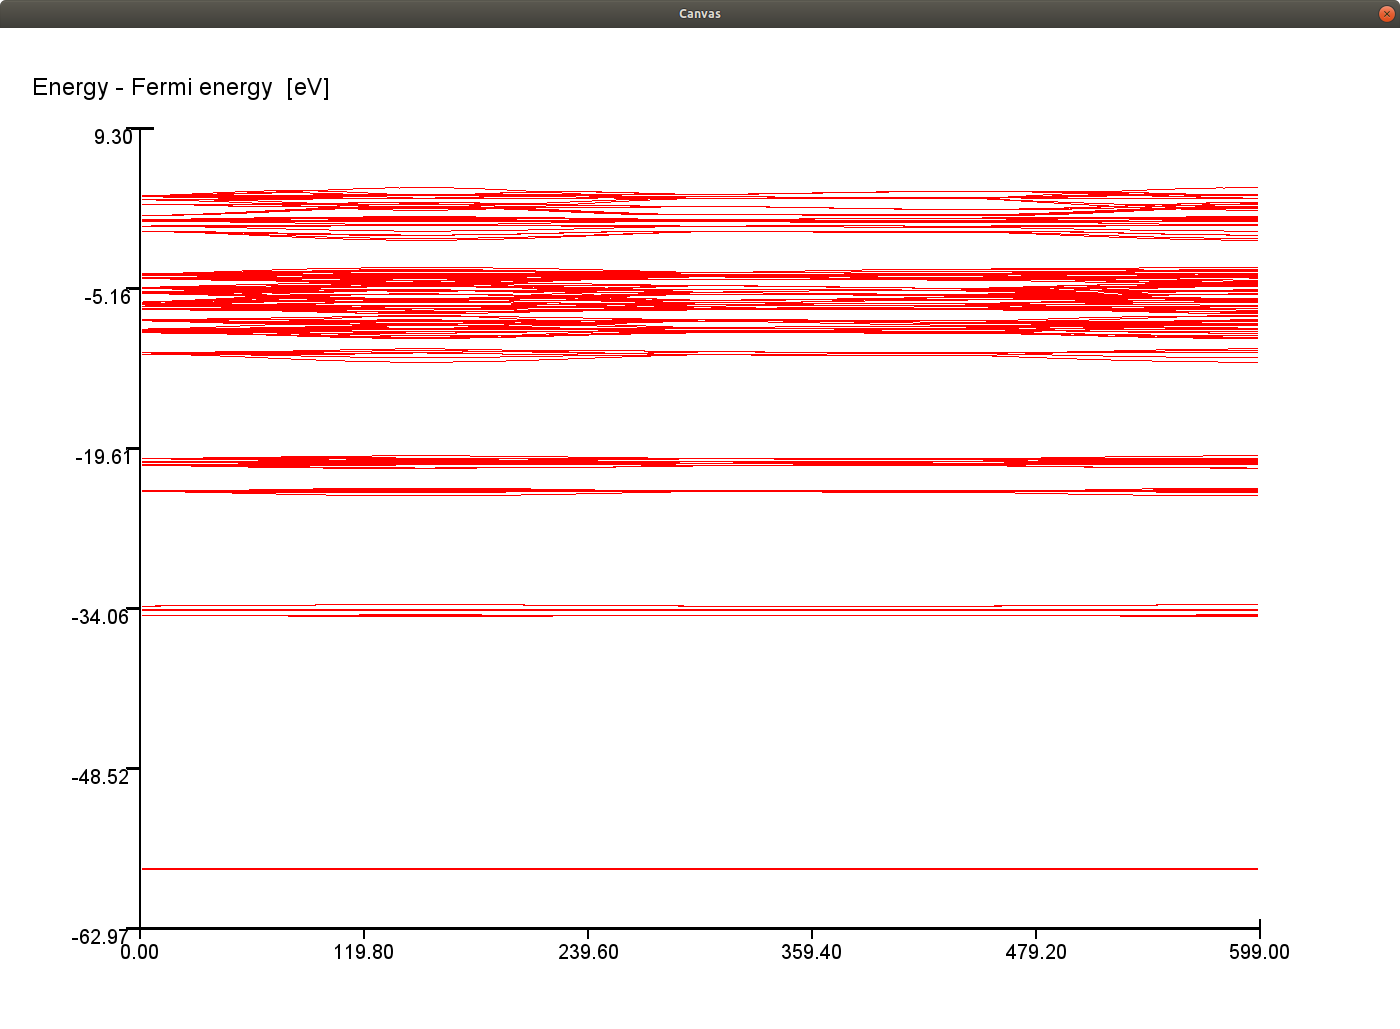
\includegraphics[width=\linewidth]{images/BandsAll.png}
        \caption{Visualisering av hela bandstrukturen som \\skapas när nätverket evalueras.}
        \label{fig:allBands}
    \end{subfigure}%
    \begin{subfigure}{.5\textwidth}
        \centering
        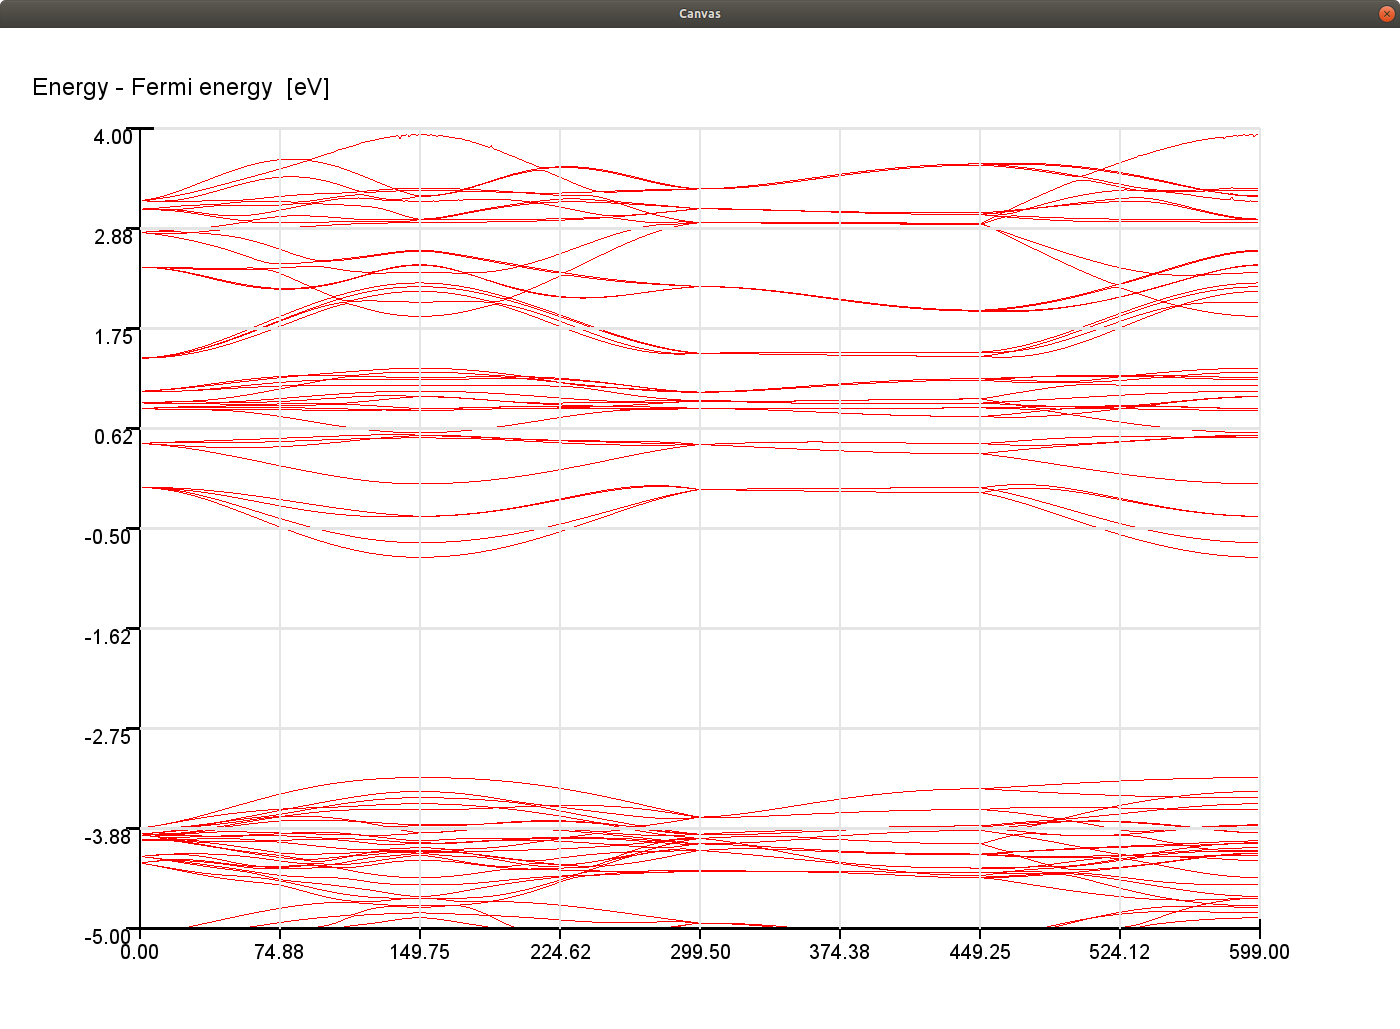
\includegraphics[width=\linewidth]{images/ZoomedBands.png}
        \caption{En förstoring av figur \ref{fig:allBands} där endast energin \\mellan $-4$ eV och $5$ eV visas.}
        \label{fig:zoomedBands}
    \end{subfigure}
    \caption{Visualisering av bandstruktur för TiPO4.}
    \label{fig:Band}
\end{figure}

\subsubsection{Tillståndstäthet}
Nätverket för visualisering av tillståndstäthetsdata laddar en \textit{HDFSource}-processor som anger HDF5-filen som data laddas från. Sedan kopplas en \textit{HDF5PathSelection}-processor, som tar ut den givna HDF5-gruppens alla undergrupper direkt till den redan befintliga \textit{HDFSource}-processorn. Denna processor anger att data ska laddas från DOS-gruppen i HDF5-filen. Två till \textit{HDF5PathSelection}-processorer laddas sedan som anger grupperna Total och Partial i HDF5-filen.  

För Total-delen laddas sedan kontinuerligt \textit{HDF5ToFunction}-processorer som gör funktioner av all 
data i Total-gruppen. För Partial-gruppen laddas en \textit{HDF5PathSelection}-processor som tar ut dataset för en vald atom genom att välja den givna HDF5-filens relevanta undergrupp. Denna processor har namnet \textit{Partial Pick} i nätverket. Därefter laddas \textit{HDF5ToFunction}-processorer för alla dataset i grupperna under Partial-gruppen. 
\newpage
All data matas sedan in i en \textit{LinePlot}-processor som gör en 2D-graf. Detta matas in i en \textit{Canvas}-processor som visar själva grafen. Dessutom finns två textOverlay processorer som skriver ut text för x- och y-axeln. Figur \ref{fig:DoS} visar total tillståndstäthet för titanfosfat, TiPO4. Figur \ref{fig:DoSNetwork} visar nätverket som ger 2D-grafen i figur \ref{fig:DoS}. Användaren kan även välja att visa en 2D-graf av den partiella tillståndstätheten med hjälp av sammma nätverk.
\begin{figure}[ht]
    \centering
    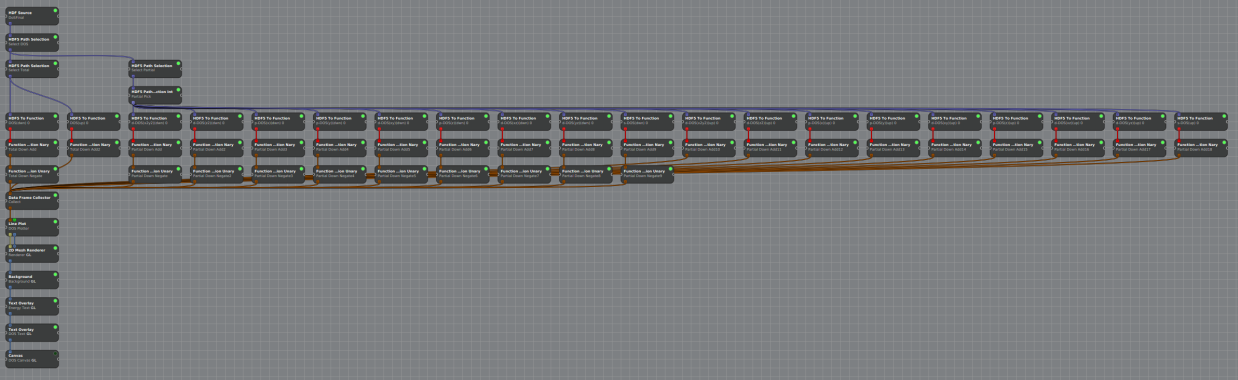
\includegraphics[angle=0, width=\linewidth]{images/DoSNetwork.PNG}
    \caption{Nätverk för visualisering av tillståndstäthet.}
    \label{fig:DoSNetwork}
\end{figure}

\begin{figure}[H]
    \begin{subfigure}{.5\textwidth}
        \centering
        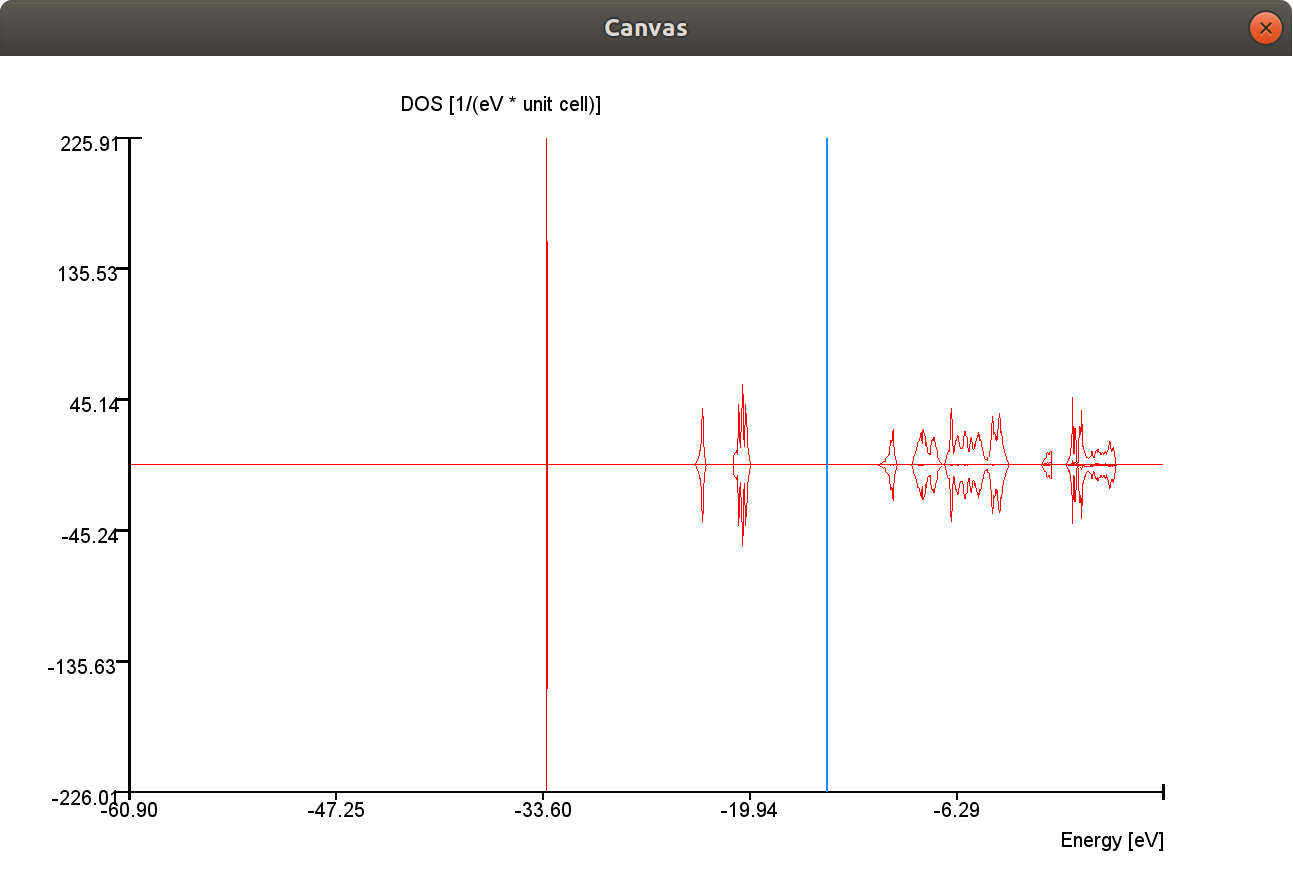
\includegraphics[width=\linewidth]{images/TotalDoS.png}
        \caption{Visualisering av den totala tillståndstätheten \\med en blå hjälplinje för avläsning.}
        \label{fig:totDoS}
    \end{subfigure}%
    \begin{subfigure}{.5\textwidth}
        \centering
        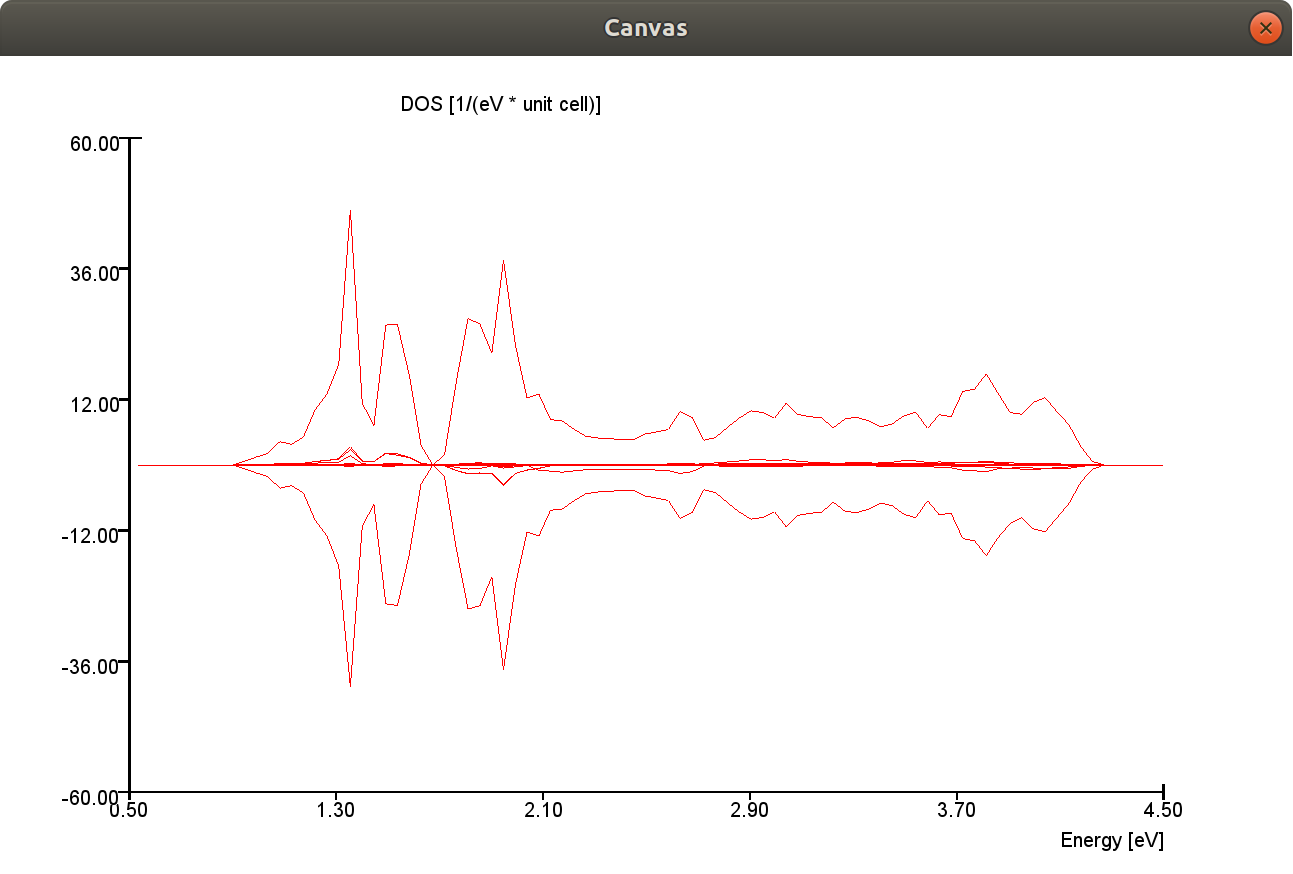
\includegraphics[width=\linewidth]{images/ZoomedDoS.png}
        \caption{Förstoring av visualiseringen av den totala \\tillståndstätheten i figur \ref{fig:totDoS}.}
        \label{fig:zoomedDoS}
    \end{subfigure}
    \caption{Visualisering av tillståndstätheten för TiPO4.}
    \label{fig:DoS}
\end{figure}

\subsection{NetworkHandlers}\label{ssec:NetworkHandlers}
För att andra delsystem enkelt ska kunna sätta upp och ändra parametrar i inviwonätverken så har python-klasser, kallade \textit{NetworkHandlers}, skrivits. Dessa klasser initierar specifika delar av nätverket och har funktioner för att ändra speciella properties i de processorer de har ansvar över. \textit{NetworkHandlers} finns för nuvarande inte för alla visualiseringar utan bara för de relaterade till volymrendering. 

\subsubsection{VolumeNetworkHandler}
En klass som sätter upp ett generiskt nätverk för volymrendering. Nätverket som byggs upp kan inte självstående ge upphåv till någon visualisering då ingen volymdatakälla initieras. Detta måste istället göras från en mer specificerad \textit{VolumeHandler}-klass som ärver denna.

\nyBild{VolumeHandler/volume_network_ex.PNG}{Nätverket som byggs upp då en VolumeNetworkHandler-instans initieras.}{VolumeNetworkHandler}{0.7}

Som visas i figur \ref{fig:VolumeNetworkHandler} så kan nätverket delas upp i två delar. En volymrenderingsdel och en tvärsnittsrenderingsdel.

Processorerna \textit{Cube Proxy Geometry}, \textit{Entry Exit Points}, och \textit{Volume Raycaster}, visade i mitten av figur \ref{fig:VolumeNetworkHandler} kommer att generera bilddata direkt baserat på den volymdata de tar emot.

Processorerna \textit{Volume Bounding Box} och \textit{Mesh Renderer} visade i högra delen av figur \ref{fig:VolumeNetworkHandler} kommer att generera bilddata av den parallellepiped som stänger in volymen. Bilddatan skickas sedan till \textit{Volume Raycaster} och sammanfogas där med bilddatan av volymen. Detta skickas sedan till \textit{Volume Background}-processorn där en bakgrund adderas till bilddatan som sedan skickas till \textit{Canvas}-processorn där den slutgiltiga visualiseringen visas.

Tvärsnittsrenderingen tar emot samma volymdata som volymrenderingen, skickar det till \textit{Volume Slice}-processorn, vilken genererar bilddata baserat på ett plan som skär volymen. Bilddatan skickas sedan till en egen canvas. Volymrenderingens \textit{Raycaster}-processor har förmågan att rita ut ett plan på en godtycklig position i volymen. Detta plan länkas till planet i \textit{Volume Slice}-processorn så att ett delvis transparent plan ritas i volymen på samma position som planet \textit{Volume Slice} använder sig av för att hämta sin data. Tvärsnittsrenderingen kan aktiveras och inaktiveras genom att dess \textit{Canvas}-processor raderas eller läggs till, och att planrenderingen i \textit{Raycaster}-processorn aktiveras eller inaktiveras.
\newpage
Viktiga funktioner i \textit{VolumeNetworkHandler}:
\begin{itemize}
    \setlength\itemsep{0em}
    \item \textbf{setup\_volume\_network: } Bygger upp nätverket som visat i figur \ref{fig:VolumeNetworkHandler}. Notera att volyminportarna ej är anslutna.
    \item \textbf{connect\_volume: } Ansluter alla volym-inportarna till en specificerad volym-outport. Detta måste göras innan en visualisering ska köras, annars har nätverket ingen volymdata att visualisera.
    \item \textbf{show\_volume\_dist: } Ritar upp ett nytt fönster med ett histogram över volymdistributionen i en specificerad HDF5-fil.
    \item \textbf{toggle\_slice\_canvas: } Tar bort eller lägger till \textit{Slice Canvas}-processorn. För att aktivera eller inaktivera tvärsnittsrenderingen.
\end{itemize}

Förutom dessa funktioner har \textit{VolumeNetworkHandler} funktioner för att ändra properties hos de processorer den initierat.

\subsubsection{UnitcellNetworkHandler}
En klass som sätter upp ett och hanterar nätverk för atompositionsrendering. Nätverket som sätts upp kan självstående generera en visualisering för bara atompotitioner men kan också kombineras med andra nätverk genom att denna ärvs i mer specificerade \textit{NetworkHandler}-klasser.

\nyBild{VolumeHandler/unitcell_network.PNG}{Nätverket som byggs upp då en UnitcellNetworkHandler-instans initieras.}{unitcell_network}{0.5}

\nyBild{VolumeHandler/unitcell_vis.PNG}{Resulterande bild från nätverk i figur\ref{fig:unitcell_network}}{unitcell_vis}{0.5}

\textit{UnitcellNetworkHandler} börjar med kontrollera att den givna HDF5-filen har data för en atompositionsvisualisering och kastar ett \textit{AssertionError} om den inte har det. Den fortsätter sedan med att sätta upp en \textit{HDF5 Source}-processor, om en sådan redan existerar så används den existerande processorn istället. Vilka atomtyper som HDF5-filen innehåller information om läses sedan. 

En \textit{Coordinate Reader}-processor för varje atomtyp  läggs till. Koordinatdatan skickas vidare till en \textit{Structure Mesh}-processor, en ENVISIoN processor som konverterar koordinaterna till en \textit{mesh}. Meshen skickas till \textit{Sphere Renderer} där den konverteras till bilddata med en sfär vid varje tidigare koordinat. Bilddatan ritas sedan ut på en \textit{Canvas}.

Viktiga funktioner i \textit{UnitcellNetworkHandler}:
\begin{itemize}
    \setlength\itemsep{0em}
    \item \textbf{setup\_unitcell\_network: } Bygger upp nätverket som visat i figur \ref{fig:unitcell_network}.
\end{itemize}

Förutom dessa funktioner har \textit{UnitcellNetworkHandler} funktioner för att ändra properties hos de processorer den initierat.


\subsubsection{ChargeNetworkHandler}
En specificerad klass för att sätta upp och hantera laddningstäthetsvisualiseringen. Klassen genererar ett fullständigt nätverk för laddningstäthetsvisualisering och har funktioner för att alla parameterändringar som där behövs. Ärver \textit{UnitcellNetworkHandler} och \textit{VolumeNetworkHandler} för att hantera atompositions- respektive volymrenderingsaspekten av visualiseringen.  

\nyBild{VolumeHandler/charge_network_ex.PNG}{Nätverket som byggs upp då en ChargeNetworkHandler-instans initieras och HDF5-filen innehåller unitcell-data.}{charge_network}{0.4}

\nyBild{VolumeHandler/charge_vis.PNG}{Resulterande bild från nätverk i figur \ref{fig:charge_network}.}{charge_vis}{0.5}

\textit{ChargeNetworkHandler} börjar med kontrollera att den givna HDF5-filen har data för en laddningstäthetsvisualisering och kastar ett \textit{AssertionError} om den inte har det. Den fortsätter sedan med att initera sina superklasser \textit{VolumeNetworkHandler} och \textit{UnitcellNetworkHandler}. Dessa sätter up sina delar av nätverket som indikerat i figur \ref{fig:charge_network}. 

En \textit{HDF5 Source} sätts upp, denna ansluts till unitcell-delen av nätverket. En \textit{HDF5 To Volume} sätts upp och anslutes till \textit{HDF5 Source}. \textit{HDF5 To Volume} hämtar ut volymdata från HDF5-filens \textit{/CHG/} sökväg. Processorn genererar volymdata som i 
sin tur ansluts med volymrenderingsdelens volymdatainportar. 

\newpage

Bilddatautporten från \textit{Sphere Renderer} ansluts till \textit{Mesh Renderer}. Detta gör att bilderna från de två processorerna slås samman och att både atompoisitoner och volymdata renderas i samma fönster. Även \textit{Sphere Renderer}-processorns \textit{Camera}-property ansluts till \textit{Mesh Renderer} för att kameravinklarna ska vara identiska.

\textit{ChargeNetworkHandler} inaktiverar som standard \textit{Slice Canvas}:en och \textit{Unitcell Canvas}:en. Dessa kan återaktiveras via sina respektive funktioner igen, exempelvis då en knapp i det grafiska gränssnittet klickas på.

Om HDF5-filen inte innehåller unitcell-data så kan \textit{UnitcellNetworkHandler} inte initieras och kastar ett exception. Endast volymrenderingsdelen av visualiseringen initieras då och atompositionsvisualiseringen ignoreras. 

Viktiga funktioner i \textit{ChargeNetworkHandler}:
\begin{itemize}
    \setlength\itemsep{0em}
    \item \textbf{setup\_charge\_network: } Bygger upp nätverket som visat i figur \ref{fig:charge_network}.
    \item \textbf{get\_available\_bands: } Returnerar en lista med de möjliga bandvalen som är möjliga i HDF5-filen.
\end{itemize}

Förutom dessa funktioner har \textit{ChargeNetworkHandler} funktioner för att ändra properties hos de processorer den initierat.

\subsubsection{ELFNetworkHandler}
ELFNetworkHandler är identisk i jämförelse med ChargeNetworkHandler med ett fåtal skillnader. Volymdata från HDF5-filen hämtas från sökvägen \textit{/ELF/} istället för \textit{/CHG/}. Detta gör att funktioner för att hämta och sätta aktiva band också är olika. 

\subsubsection{ParchgNetworkHandler}
En specificerad klass för att sätta upp och hantera visualiseringen för partiell laddningstäthet. Ärver \textit{VolumeNetworkHandler} och \textit{UnitcellNetworkHandler} för att hantera volymrenderingsaspekten respektive atompositionsaspekten av visualiseringen.


\nyBild{VolumeHandler/parchg_network_ex.png}{Nätverket som byggs av ParchgNetworkHandler (utan atompositionsrendering).}{parchg_network}{0.6}

Till att börja med initieras superklassen \textit{VolumeNetworkHandler} detta sätter upp det generiska volymrenderingsnätverket. 

Efter detta initieras volymdatakällan och volymdataoutporten ansluts till volymrenderingsdelen av nätverket. 

Volymkällan är här mer komplicerad i jämförelse mot övriga visualiseringar, eftersom flera olika volymdataset här ska visualiseras som en volym. Precis hur denna del ser ut beror på de bandval som görs av användaren.

\nyBild{VolumeHandler/parchg_source_ex.png}{Exempel på nätverkets volymdatakälla med ett bandval för varje läge.}{parchg_source}{0.5}

Den partiella laddningstäthetsvisualiseringen tillåter användaren att välja ett godtyckligt antal band som ska visualiseras och ett av fyra olika lägen för varje band. Dessa lägen är \textit{Total}, \textit{Magnetic}, \textit{Up-spin}, och \textit{Down-spin}. De olika lägena hämtar ut volymdata ur HDF5-filen på olika sätt.

\begin{itemize}
    \setlength\itemsep{0em}
    \item \textbf{Total: } Hämtar direkt volymdatan från det valda bandets \textit{/total/} sökväg.
    \item \textbf{Magnetic: } Hämtar direkt volymdatan från det valda bandets \textit{/magnetic/} sökväg.
    \item \textbf{Up-spin: } Hämtar ut både \textit{/total/} och \textit{/magnetic/} volymdatan som \textit{v1} och \textit{v2}. Volymerna summeras sedan med formeln \textit{0.5*(v1+v2)}
    \item \textbf{Down-spin: } Hämtar ut både \textit{/total/} och \textit{/magnetic/} volymdatan som \textit{v1} och \textit{v2}. Volymerna summeras sedan med formeln \textit{0.5*(v1-v2)}
\end{itemize}

Volymdatan från de olika bandvalen kombineras sedan med en \textit{Volume Merger}-processor. \textit{Volume Merger} kan summerar upp till fyra volymer till en. Om mer än fyra bandval har gjorts så används flera lager av \textit{Volume Merger}-processorer för att kunna summera alla dessa till en. Volymdatan från den sista \textit{Volume Merger} skickas sedan till volymrenderingsnätverket.

Viktiga funktioner i \textit{ParchgNetworkHandler}:
\begin{itemize}
    \setlength\itemsep{0em}
    \item \textbf{setup\_hdf5\_source: } Initierar \textit{HDF Source}-processorn
    \item \textbf{setup\_band\_processors: } Sätter upp nätverket som hämtar ut och kombinerar volymdata baserat på bandval och lägen. Funktionen kan kallas flera gånger efter att nätverket har startats för att byta bandval och lägen.
\end{itemize}

\newpage

\subsubsection{Plannerade NetworkHandlers}
NetworkHandler-klasser har inte skrivits för alla visualiseringar, de gamla visualiseringsskripten används fortfarande för att starta de tvådimensionella visualiseringarna. För att underlätta underhåll av systemet så bör dessa färdigställas i framtiden. I nuläget finns funktionaliteten för att starta och styra dessa visualiseringar utspridd mellan flera olika filer på olika platser. 
\begin{itemize}
    \setlength\itemsep{0em}
    \item \textbf{LinePlotNetworkHandler: } Skulle hantera den generella delen av en 2D-graf visualisering. Styr allt som har med 2D-grafen att göras, som skalning, axlar på grafen, med mera.
    \item \textbf{BandstructureNetworkHandler: } Ärver LinePlotNetworkHandler och sätter upp den specifika delen för bandstructure visualiseringen. Skulle styra HDF5-källan och  bandval.
    \item \textbf{DOSNetworkHandler: } Ärver LinePlotNetworkHandler och UnitcellNetworkHandler och sätter upp den specifika delen för tillståndstäthets visualiseringen. Skulle styra HDF5-källan och val av tillstånd.
    \item \textbf{PCFNetworkHandler: } Ärver LinePlotNetworkHandler och sätter upp den specifika delen för parkorrelationsfunktions visualiseringen.Skulle styra HDF5-källan och val av tidssteg.
\end{itemize}

\newpage
\subsection{Datastrukturer}
\label{ssec:datastrukturer}
Två datastrukturer, Point och Function, har introducerats. En datastruktur är en form av behållare av olika typer av data som kan skickas mellan processorer. Dessa används i vissa av de implementerade processorerna.
\subsubsection{Point}
Denna datatyp representerar en reell 1D-punkt och inkapslar punktens värde (ett flyttal) samt variabel metadata.
\subsubsection{Function}
Denna datatyp representerar en reellvärd funktion av en reell variabel och inkapslar sampelvärden och variabel-metadata för x- och y-axlarna.

\subsection{Processorer}
\label{ssec:processorer}
För att kunna omvandla den data som översatts från VASP-beräkningar till en visualisering krävs processorer som utför specifika uppgifter. Figur 2 demonstrerar ett typiskt utseende på en processor.
\nyBild{processor.png}{Exempel på en processors utseende.}{processor}{0.8}
De färgade rutorna till vänster på processorn i figur \ref{fig:processor} är olika typer av ingångar och utgångar. Cirkeln i det övre högra hörnet på processorn i samma figur är en lampa som lyser då processorn är aktiv. De processorer som ENVISIoN skapat kategoriseras och beskrivs nedan.

\subsubsection{Kristallstruktur}
\label{ch:kristallstruktur-processorer}
Nedanstående processorer är relaterade till visualiseringen av kristallstrukturer. De tillhör en modul vid namn Crystalvisualization.

\textbf{\textit{CoordinateReader}} \newline
Från en HDF5-fil läser denna processor koordinater för atompositioner. En sökväg till ett dataset sätts via en StringProperty. Utdata från CoordinateReader är $n$ stycken vec3.

Inport:
\begin{itemize}
\item Hdf5::Inport inport\_
\end{itemize}

Utport:
\begin{itemize}
\item DataOutport< std::vector<vec3> > outport\_
\end{itemize}

Properties:
\begin{itemize}
\item StringProperty path\_
\end{itemize}

\textbf{\textit{StructureMesh}} \newline
Atompostionsdata kopplas ihop med rätt atomfärg och radie med StructureMesh-processorn. StructureMesh har en multiinport, dit en eller flera CoordinateReader-processorer kan kopplas in. Indata för StructureMesh är atompositionsdata i form av vec3 för varje atomslag. Till denna indata läggs properties för färg, radie och antal till för varje atomslag/processor som kopplas in. Den ger en mesh, som har buffrar för position, färg och radie.

Inport:
\begin{itemize}
\item DataInport< std::vector<vec3>, 0> structure\_
\end{itemize}

Utport:
\begin{itemize}
\item MeshOutport mesh\_
\end{itemize}

Properties:
\begin{itemize}
    \setlength\itemsep{0em}
    \item FloatProperty scalingFactor\_
    \item FloatMat3Property basis\_
    \item BoolProperty fullMesh\_
    \item IntProperty timestep\_
    \item std::vector< std::unique\_ptr<FloatVec4Property> > colors\_: vektor som innehåller färgproperty för varje atomslag
    \item std::vector< std::unique\_ptr<FloatProperty > > radii\_: vektor som innehåller radieproperty för varje atomslag
    \item std::vector< std::unique\_ptr<IntProperty> > num\_: vektor som innehåller antalet atomer per tidssteg för varje atomslag
    \item BoolProperty enablePicking\_: sann då picking-funktionen är påslagen 
    \item IntVectorProperty inds\_: vektor med index på valda atomer
\end{itemize}

\subsubsection{HDF5}
\label{ch:hdf5-processorer}
Nedanstående processorer är ämnade att fungera väl med de HDF5-relaterade processorer som är inkluderade i Inviwo.

\textbf{\textit{HDF5PathSelection*}} \newline
Detta är en grupp av processorer som har funktionalitet liknande den inbyggda processorn HDF5PathSelection. En eller flera av dessa processorer placeras med fördel mellan en HDFSource och en eller flera HDF5To*.

Gemensamt för dessa processorer är  att de på inporten tar en Hdf5-grupp och på utporten skriver noll eller flera av dessa omedelbara undergrupper.

Nedan beskrivs de olika processorerna i denna grupp.

\textbf{HDFpathSelectionInt} \newline
Denna processor väljer en HDF5-grupp med heltalsnamn, baserat på värdet på processorns intProperty\_, eventuellt utökat med ledande nollor till bredden specificerat på processorns zeroPadWidthProperty\_.

HDF5PathSelectionInt kan med fördel användas tillsammans med en OrdinalPropertyAnimator för att plocka ut relevant data ur en HDF5-fil.

Anledningen till att utdata ges som en vektor av HDF5-grupper, trots att processorn alltid skriver exakt en grupp på utporten, är att processorn ska följa samma mönster som, och fungera väl med, resterande processorer.

Inport:
\begin{itemize}
\item DataInport<hdf5::Handle> hdf5HandleInport\_
\end{itemize}

Utport:
\begin{itemize}
\item DataOutport< std::vector<hdf5::Handle> > hdf5HandleVectorOutport\_
\end{itemize}

Properties:
\begin{itemize}
    \setlength\itemsep{0em}
    \item IntProperty intProperty\_
    \item IntSizeTProperty zeroPadWidthProperty\_
\end{itemize}

\textbf{HDF5PathSelectionIntVector} \newline
Denna processor väljer noll eller flera HDF5-grupper med heltalsnamn, baserat på värdet på processorns intVectorProperty\_, eventuellt utökat med ledande nollor till berdden specificerat av processorns zeroPadWidthProperty\_. 

HDF5PathSelectionIntVector kan med fördel användas tillsammans med ''picking'' för att plocka ut relevant data ur en HDF5-fil.

Inport:
\begin{itemize}
\item DataInport<hdf5::Handle> hdf5HandleInport\_
\end{itemize}

Utport:
\begin{itemize}
\item DataOutport< std::vector<hdf5::Handle> > hdf5HandleVectorOutport\_
\end{itemize}

Properties:
\begin{itemize}
    \setlength\itemsep{0em}
    \item IntVectorProperty intVectorProperty\_
    \item IntSizeTProperty zeroPadWidthProperty\_
\end{itemize}

\textbf{HDF5PathSelectionAllChildren}\newline
Denna processor väljer den givna HDF5-gruppens alla undergrupper.

Inport:
\begin{itemize}
\item DataInport<hdf5::Handle> hdf5HandleInport\_
\end{itemize}

\textbf{\textit{HDF5To*}}\newline
Detta är en grupp av processorer som har funktionalitet liknande den inbyggda processorn HDF5ToVolume. Processorerna placeras med fördel efter en HDFSource-processor, med en eller flera mellan liggande HDF5PathSelection*.

Gemensamt för dessa är att de som indata tar noll eller flera HDF5-grupper (baserat på *pathSelectionProperty\_), plockar ut dataset för varje grupp och omvandlar dessa till relevanta objekt (Point eller Function) som sedan skrivs till utporten. Objektens variabel-metadata tas, om de finns tillgängliga, från attributen associerade med dataseten. Vidare kan, om så väljs med *namePrependParentsProperty\_, metadat utökas med namnen på de grupper var i dataseten ligger.

Vilka dataset som kan väljas med *pathSelectionProperty\_ uppdateras dynamiskt beroende på vilka grupper som ligger på inporten. När ett lämpligt dataset valts kan *pathFreezeProperty\_ användas för att stänga av denna dynamik, så att värdet sparas även om grupperna på inporten (antagligen tillfälligt) ändras. Detta underlättar manuellt experimenterande samt användandet av processorer som tillfälligt ger noll grupper som utadat, t.ex. HDF5PathSelectionIntVector.

\textbf{HDF5ToPoint} \newline
Denna processor konverterar HDF5-data till noll eller flera Point-objekt.

Inport:
\begin{itemize}
\item DataInport<hdf5::Handle, 0, true> hdf5HandleFlatMultiInport\_
\end{itemize}

Utport:
\begin{itemize}
\item DataOutport< std::vector<Point> > pointVectorOutport\_
\end{itemize}

Properties:
\begin{itemize}
    \setlength\itemsep{0em}
    \item OptionPropertyString pathSelectionProperty\_
    \item BoolProperty pathFreezeProperty\_
    \item IntSizeTProperty namePrependParentsProperty
\end{itemize}

\textbf{HDF5ToFunction}\newline
Denna processor konverterar HDF5-data till noll eller flera Function-objekt. 

Normalt plockas två dataset per grupp ut, ett för x-axeln och ett för y-axeln. Om endast data för y-axeln finns tillgänglig kan implicitXProperty\_ sättas, varvid processorn automatgenererar data för x-axeln.

Inport:
\begin{itemize}
\item DataInport<hdf5::Handle, 0, true> hdf5HandleFlatMultiInport\_
\end{itemize}

\newpage

Utport:
\begin{itemize}
\item DataOutport< std::vector<Function> > functionVectorOutport\_
\end{itemize}

Properties:
    \begin{itemize}
    \setlength\itemsep{0em}
    \item BoolProperty implicitXProperty\_
    \item OptionPropertyString xPathSelectionProperty\_
    \item OptionPropertyString yPathSelectionProperty\_
    \item BoolProperty xPathFreezeProperty\_
    \item BoolProperty yPathFreezeProperty\_
    \item IntSizeTProperty xNamePrependParentsProperty\_
    \item IntSizeTProperty yNamePrependParentsProperty\_
\end{itemize}

\subsubsection{2D}
\label{ch:2d-processorer}
Nedanstående processorer är ämnade att bearbeta och presentera 2D-data, närmare bestämt data av typen Point och Function.

\textbf{\textit{FunctionOperationUnary}}\newline
Denna processor implementerar en unär operator, antingen negation $(g_{i}(x) = -f_{i}(x))$ eller (multiplikativ) inversion $(g_{i}(x) = 1/f_{i}(x))$. Operatorn appliceras på funktioner på inporten, en i taget, och skriver respektive resultat på utporten.

Inport:
\begin{itemize}
\item DataFrameInport dataframeInport\_
\end{itemize}

Utport:
\begin{itemize}
\item DataFramOutport dataframOutport\_
\end{itemize}

Properties:
\begin{itemize}
\item OptionPropertyString operationProperty\_
\end{itemize}

\textbf{\textit{FunctionOperationNary}}\newline
Denna processor implementerar en operator med variabel aritet (engelska n-ary), antingen addition/summa $(g(x) = \Sigma_{i}f_{i}(x))$ eller multiplikation/produkt $(g(x) = \Pi_{i}f_{i}(x))$. Operatorn appliceras på samtliga funktioner på inporten och skrver resultatet på utporten.

Då funktionerna på inporten kan vara samplade vid olika x-värden behöver processorn ta beslut om var ut-funktionen ska samplas. Processorn utgår från att sampla i samtliga x-värden för samtliga in-funktioner. sampleFilterEnableProperty\_ kan sättas för att filtrera dessa. Då sampleFilterEnableProperty\_ är satt ser processorn till att sampelavståndet är minst det värde som anges i sampleFilterEpsilonProperty\_. När processorn skapas är sampleFilterEnableProperty\_ satt och sampleFilterEpsilonProperty\_ är 0 vilket innebär att x-värden som är identiska filtreras bort.

Om ett värde behöver beräknas vid ett x-värde där en in-funktion inte är samplat används linjär interpolation om x-värdet ligger innanför funktionens definitionsintervall. Om x-värdet ligger utanför detta intervall används undefinedFallbackProperty\_ för att avgöra vilket värde som används istället. Detta kan antingen vara noll eller funktionens värde vid intervallets relevanta ändpunkt.

Inport
\begin{itemize}
\item org.envision.FunctionFlatMultiInport functionFlatMultiInport\_ 
\end{itemize}

Utport:
\begin{itemize}
\item DataFramOutport dataframOutport\_
\end{itemize}

Properties:
\begin{itemize}
    \setlength\itemsep{0em}
    \item OptionsPropertyString operationProperty\_
    \item OptionsPropertyString undefinedFallbackProperty\_
    \item BoolProperty sampleFilterEnableProperty\_
    \item FloatProperty sampleFilterEpsilonProperty\_
\end{itemize}

\textbf{\textit{LinePlot}}\newline
LinePlot tar en \emph{DataFrame} som förväntas innehålla minst två kolumner med data. Den konstruerar en mesh som
representerar en linjegraf. Denna mesh renderas sedan, förslagsvis med hjälp av en \emph{2D Mesh Renderer}-processor för att generera en bild av grafen.

LinePlot genererar även en utbild att lägga över grafen som innehåller axelgraderingen. Axelgraderingen kan också den skickas in i \emph{2D Mesh Renderer}-processorn och kommer då läggas ovanpå grafen.

Användaren väljer vilken kolumn i den \emph{DataFrame} som processorn tar in som ska representeras på vardera axel genom val i \textit{xSelectionProperty\_} och \textit{ySelectionProperty\_}. Vill användaren välja multipla kolumner som ska representeras på y-axeln sätts \textit{boolYSelection\_} till sant för att sedan välja vilka kolumner i med hjälp av en sträng i \textit{groupYSelection\_}. Användaren kan även välja alla kolumner som inte representeras på x-axeln att representeras på y-axeln genom att sätta \textit{allYSelection\_} till sant.

Inställningar som har \emph{range} i namnet justerar minimum- och
maximumvärden på koordinataxlarna. Inställningar med \emph{width}
eller \emph{colour} justerar bredd respektive färg för olika linjer ritade i diagrammet.

\emph{label\_number\_} anger antalet divisioner på koordinataxlarna. Är värdet till exempel satt till tjugo innebär det att varje axel kommer ha tjugo divisioner och tjugo axelgraderingsetiketter, utöver de etiketter på startvärdena på vardera axel.

\emph{font\_} ställer in vilket typsnitt axelgraderingen skall ha.

\emph{enable\_line\_} aktiverar ritandet av en vertikal linje på
x-koordinaten specificerad i \emph{line\_x\_coordinate\_}. Denna är avsedd att ge en visuell markering av var specifika x-värden finns på x-axeln.

\newpage

Inport:
\begin{itemize}
    \setlength\itemsep{0em}
    \item DataFrameInport dataFrameInport\_
    \item DataInport<Point, 0, true> pointInport\_
\end{itemize}

Utports:
\begin{itemize}
    \setlength\itemsep{0em}
    \item MeshOutport meshOutport\_
    \item ImageOutport labels\_
\end{itemize}

Properties:
\begin{itemize}
    \setlength\itemsep{0em}
    \item OptionPropertyString xSelectionProperty\_
    \item OptionPropertyString ySelectionProperty\_
    \item StringProperty groupYSelection\_
    \item BoolProperty boolYSelection\_
    \item BoolProperty allYSelection\_
    \item FloatVec4Property colour\_
    \item FloatVec2Property x\_range\_
    \item FloatVec2Property y\_range\_
    \item FloatProperty scale\_
    \item BoolProperty enable\_line\_
    \item FloatProperty line\_x\_coordinate\_
    \item FloatVec4Property line\_colour\_
    \item BoolProperty show\_x\_labels\_
    \item BoolProperty show\_y\_labels\_
    \item FloatVec4Property axis\_colour\_
    \item FloatProperty axis\_width\_
    \item BoolProperty enable\_grid\_
    \item FloatVec4Property grid\_colour\_
    \item FloatProperty grid\_width\_
    \item FontProperty font\_
    \item FloatVec4Property text\_colour\_
    \item IntProperty label\_number\_
\end{itemize}

\textit{\textbf{DataFrameCollector}}\\
Processorn utför inga beräkningar, utan den samlar endast ihop DataFrame från ett godtyckligt antal andra processorer till endast en DataFrame. Behovet för denna processor dök upp då visualiseringen för tillståndstäthet uppdaterades. Önskan att välja specifika partiella tillstånd kunde uppfyllas med hjälp av denna processor.

\newpage

Inport:
\begin{itemize}
    \item DataInport<DataFrame, 0> dataframeInport\_
\end{itemize}

Utport:
\begin{itemize}
    \item DataFrameOutport dataframeOutport\_
\end{itemize}

\textit{\textbf{FunctionToDataFrame}}\\
Denna processor extraherar data från funktioner till en DataFrame där varje funktion ger upphov till två kolumner. All data i en funktion har även information om densamma, t.ex. variabelnamn och enhet. Namnet på vardera kolumn som skapas är dess variabelnamn från funktionen. 

Processorn skapades då det tidigare inte funnits ett sätt att extrahera data från flera funktioner samtidigt. Då har lösningen varit att använda en processor för varje funktion som har data att extrahera. Problematiken med den lösningen är att en visualisering kan vara väldigt tidskrävande. En visualisering av bandstruktur kan potentiellt ha flera hundra funktioner. Med FunctionToDataFrame kan detta göras med endast en processor.

Inport:
\begin{itemize}
    \item DataInport<Function, 0, true> functionFlatMultiInport\_
\end{itemize}

Utport:
\begin{itemize}
    \item DataFrameOutport dataframeOutport\_
\end{itemize}

\subsection{Properties och widgets}
\label{ssec:Properties}
\subsubsection{IntVectorpropety}
Denna property består av en vektor av int-värden.
\subsubsection{IntVectorPropertyWidget}
En widget för IntVectorProperty. ''Textbox'', satt till endast läsning (read only), som innehåller de värden som finns i tillhörande IntVectorProperty.
\newpage
\section{Using Legacy GUI}
\label{sec:GUI}
ENVISIoN is equipped with a graphical user interface to simplify the usage of ENVISIoN. 

\subsection{Start-up}
When the user starts the application through a computer terminal (see chapter \ref{sec: start envision}) a window opens, see figure \ref{fig:GUIStartupUbuntu} for Ubuntu and figure for Windows. The start-up window of ENVISIoN has a sidebar menu to the left with different choices. Each choice has its own content to the right. By default, the ``Dataset loader'', is chosen from start. The other possible choices are ``Parser'' or ``About''. Under ``Active datasets'' the loaded datasets will appear. Each alternative will be explained in their own sections in this chapter. The following figures of the GUI in this chapter will be for Windows but the content is the same for every operative system.

\begin{figure}[H]
    \centering
    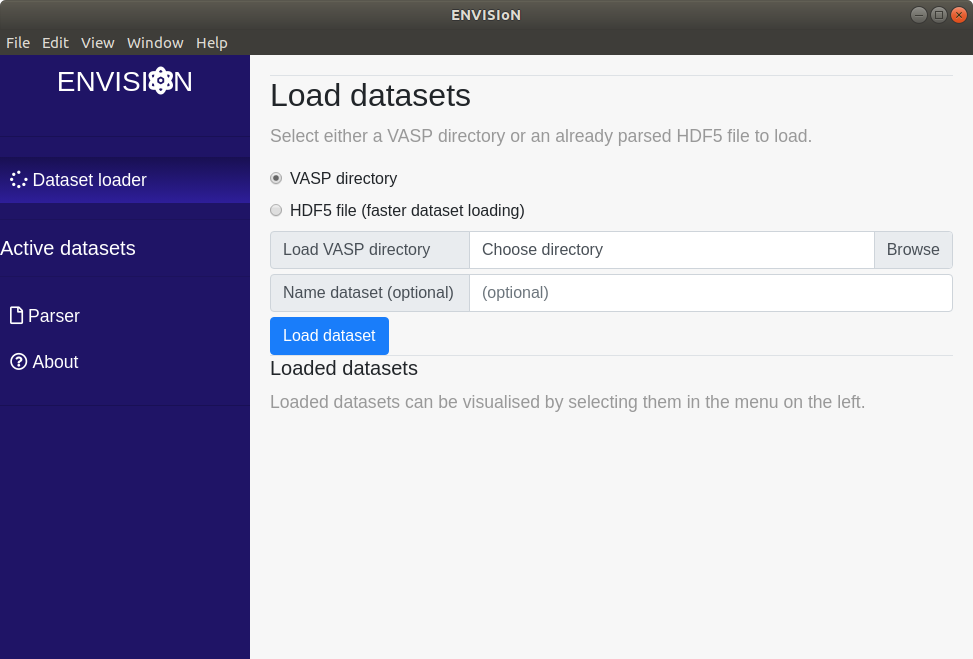
\includegraphics[scale = 0.3]{Images/GUI_start_Ubuntu.png}
    \caption{ENVISIoN start-up window for Linux.}
    \label{fig:GUIStartupUbuntu}
\end{figure}

\begin{figure}[H]
    \centering
    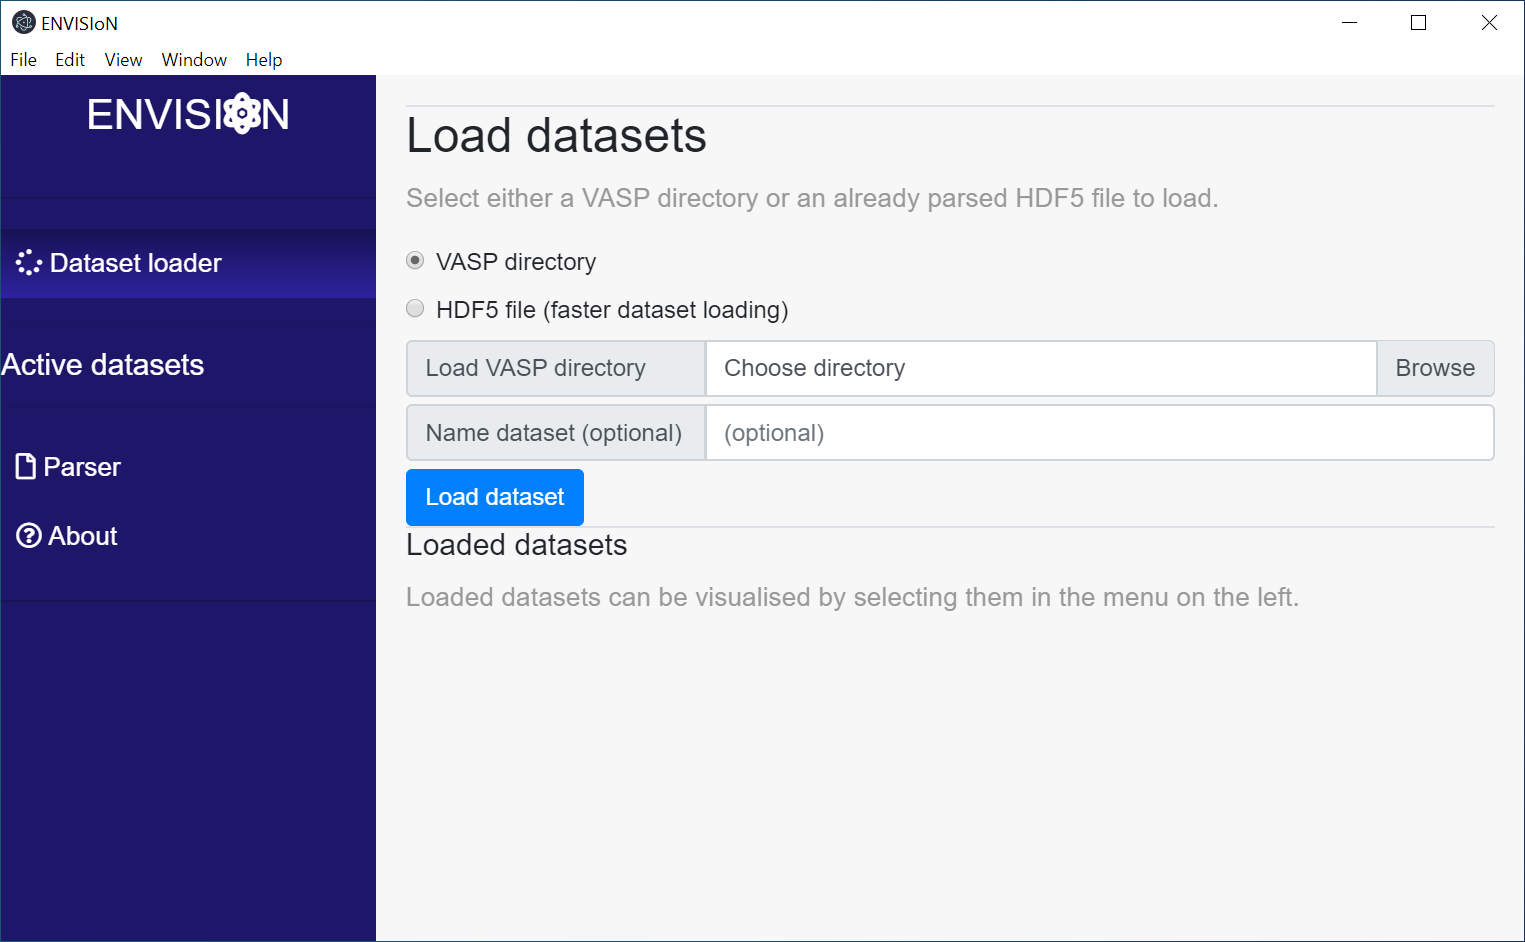
\includegraphics[scale = 0.4]{Images/GUI_start_Windows.png}
    \caption{ENVISIoN start-up window for Windows.}
    \label{fig:GUIStartupUbuntu}
\end{figure}

\subsection{Dataset loader}
In the ``Dataset loader'' a user can select either a VASP file or a HDF5 file to load which then will be visualised. To load a VASP file, the box ``VASP directory'' need to be checked. To load a HDF5 file the box ``HDF5 file'' need to be checked. 

For a quick step-by-step guide, scroll down to section \ref{sec:Dataset step-by-step}.

\subsubsection{Load a VASP file}
For loading a VASP file, the content for the ``Dataset loader'' is shown below in figure \ref{fig:GUIDatasetloaderVASP}.

\begin{figure}[H]
    \centering
    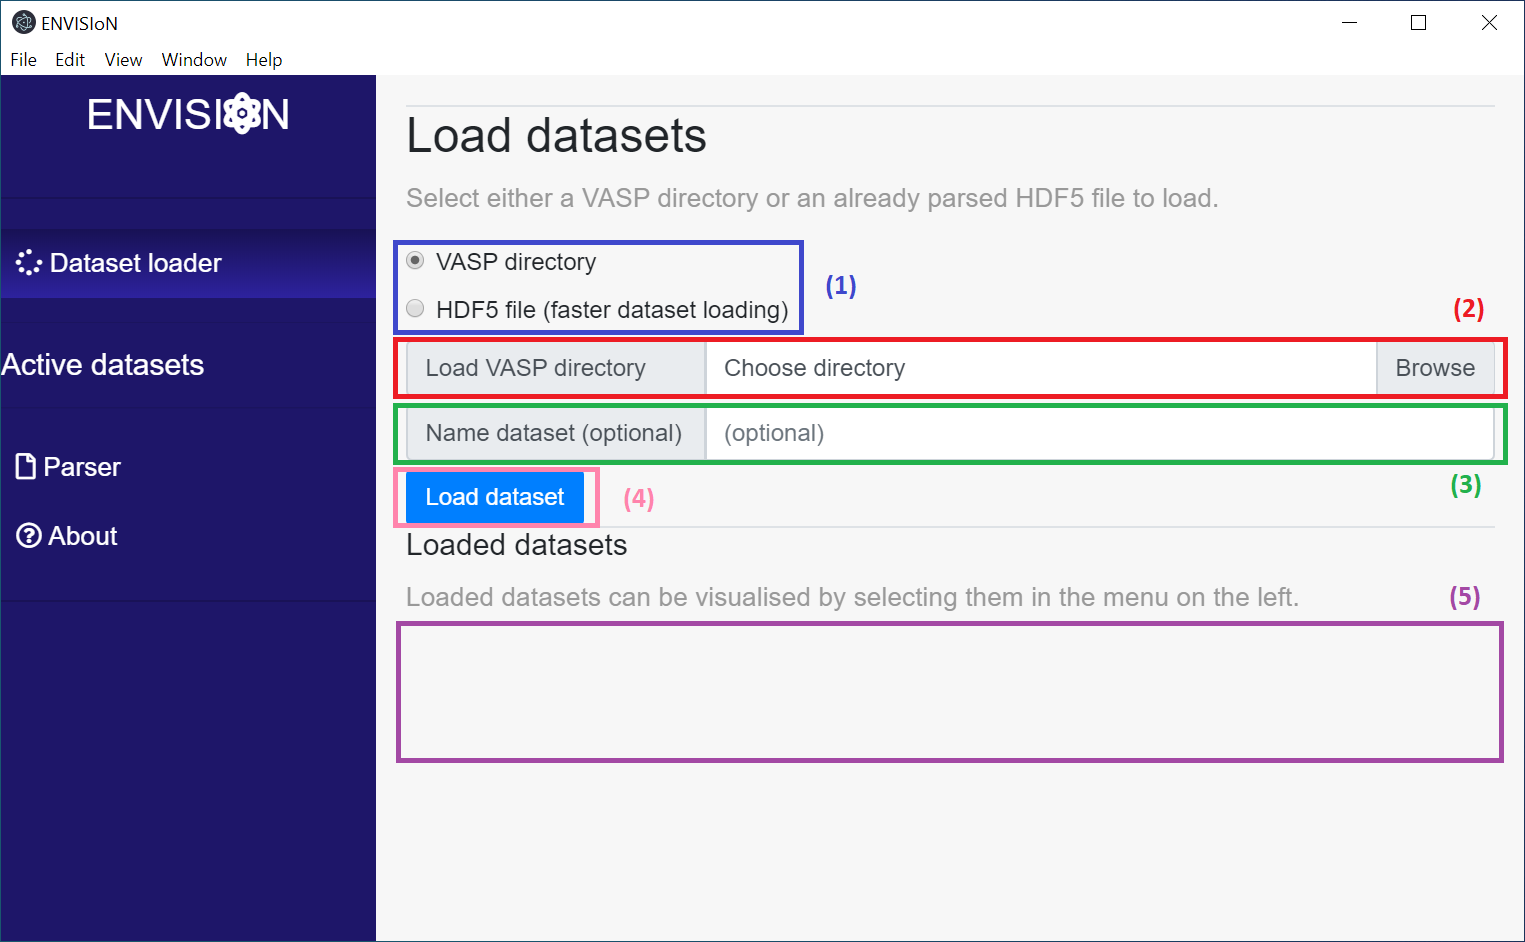
\includegraphics[scale = 0.45]{Images/GUI_Datasetloader_VASP.png}
    \caption{Dataset loader for VASP source.}
    \label{fig:GUIDatasetloaderVASP}
\end{figure}

In the blue box labeled (1) the box ``VASP directory'' need to be checked. In the red box labeled (2) the path to the VASP directory to load is selected. By clicking on ``Browse'' a new window will appear where the user navigates to the VASP directory on the computer and selects it. In the green box labeled (3) the user can write a name for the dataset. This is optional. In the pink box labeled (4) is the ``Load dataset'' button. When pressing this button the dataset will be loaded. The loaded dataset will be displayed in the purple box labeled (5) and in the sidebar menu under ``Active datasets''.

\subsubsection{Load a HDF5 file}
For loading a HDF5 file, the content for the ``Dataset loader'' is shown below in figure \ref{fig:GUIDatasetloaderHDF5}.

\begin{figure}[H]
    \centering
    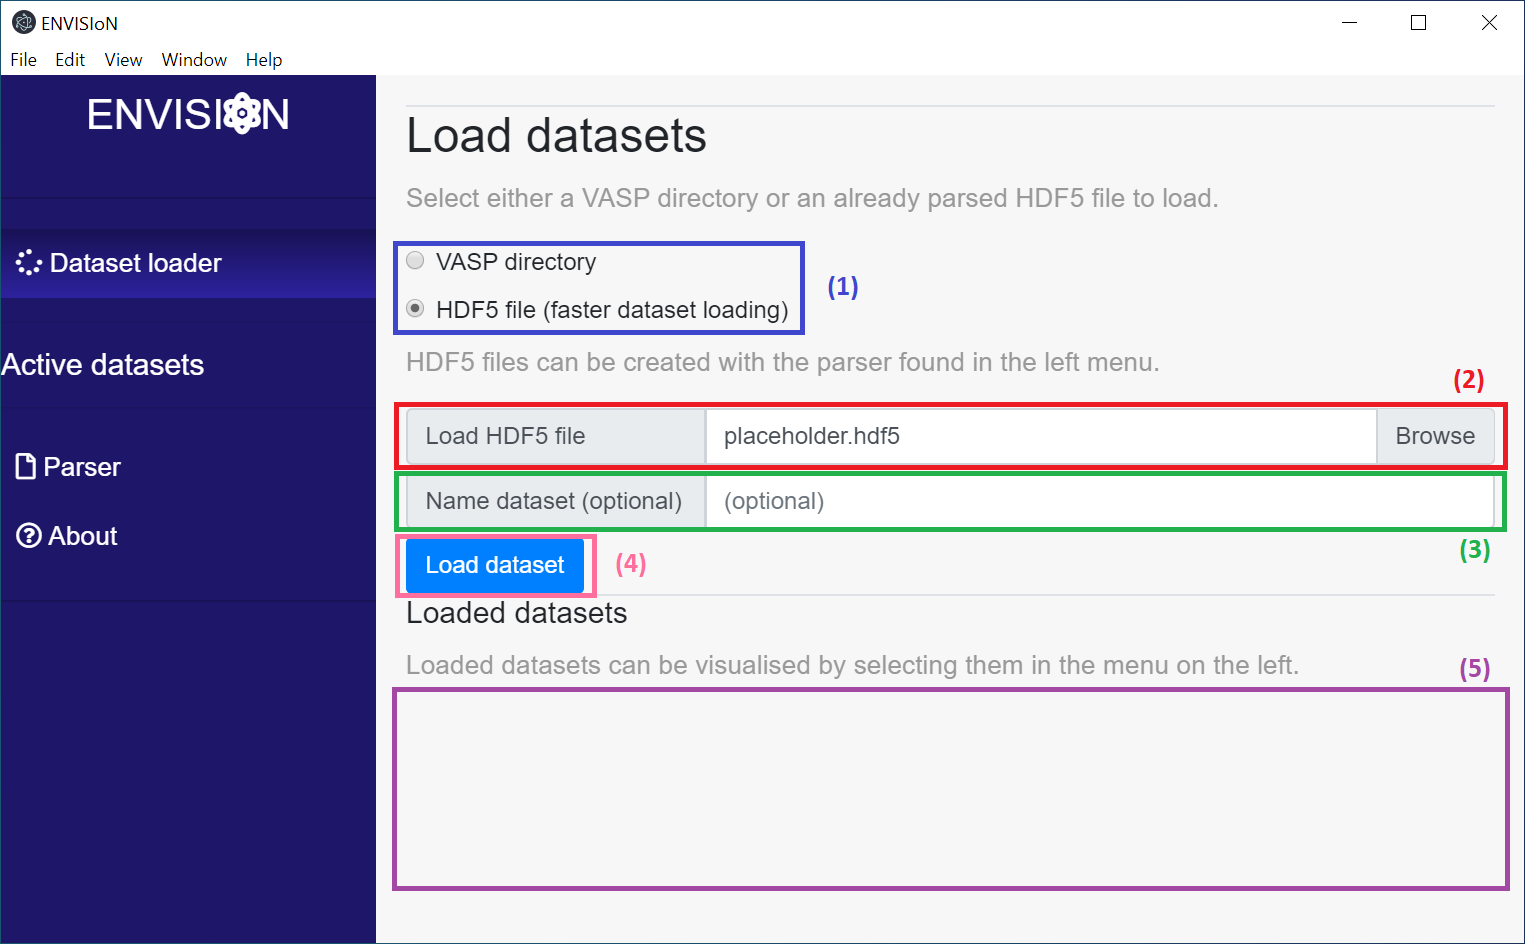
\includegraphics[scale = 0.45]{Images/GUI.Datasetloader_HDF5.png}
    \caption{Dataset loader for HDF5 source.}
    \label{fig:GUIDatasetloaderHDF5}
\end{figure}

In the blue box labeled (1) the box ``HDF5 file'' need to be checked. In the red box labeled (2) the path to the HDF5 file to load is selected. By clicking on ``Browse'' a new window will appear where the user navigates to the HDF5 file on the computer and selects it. In the green box labeled (3) the user can write a name for the dataset. This is optional. In the pink box labeled (4) is the ``Load dataset'' button. When pressing this button the dataset will be loaded. The loaded dataset will be displayed in the purple box labeled (5) and in the sidebar menu under ``Active datasets''.

\subsubsection{Quick Step-by-step guide}
\label{sec:Dataset step-by-step}
To load a VASP-file (referring to figure \ref{fig:GUIDatasetloaderVASP}):
\begin{enumerate}
    \item Check the box ``VASP directory'' in (1).
    \item Choose a VASP directory on your computer by clicking ``Browse'' in (2).
    \item (optional) Name the dataset by writing in (3).
    \item Click ``Load dataset'' in (4).
    \item Now the loaded dataset is showing in (5) and in the sidebar menu under ``Active datasets''.
\end{enumerate}

To load a HDF5 file (referring to figure \ref{fig:GUIDatasetloaderHDF5}):
\begin{enumerate}
    \item Check the box ``HDF5 file'' in (1).
    \item Choose a HDF5 file on your computer by clicking ``Browse'' in (2).
    \item (optional) Name the dataset by writing in (3).
    \item Click ``Load dataset'' in (4).
    \item Now the loaded dataset is showing in (5) and in the sidebar menu under ``Active datasets''.
\end{enumerate}

\subsection{Active datasets}
When a dataset is loaded for visualisation it will appear under ``Active datasets'' in the sidebar menu. 

\subsubsection{Starting the visualisation}
By clicking on one of datasets under ``Active datasets'', new content will show up to the right, see figure \ref{fig:GUIChosevistype} below. In figure \ref{fig:GUIChosevistype} the dataset ``BaSO4\_ORC'' is loaded as an example.

\begin{figure}[H]
    \centering
    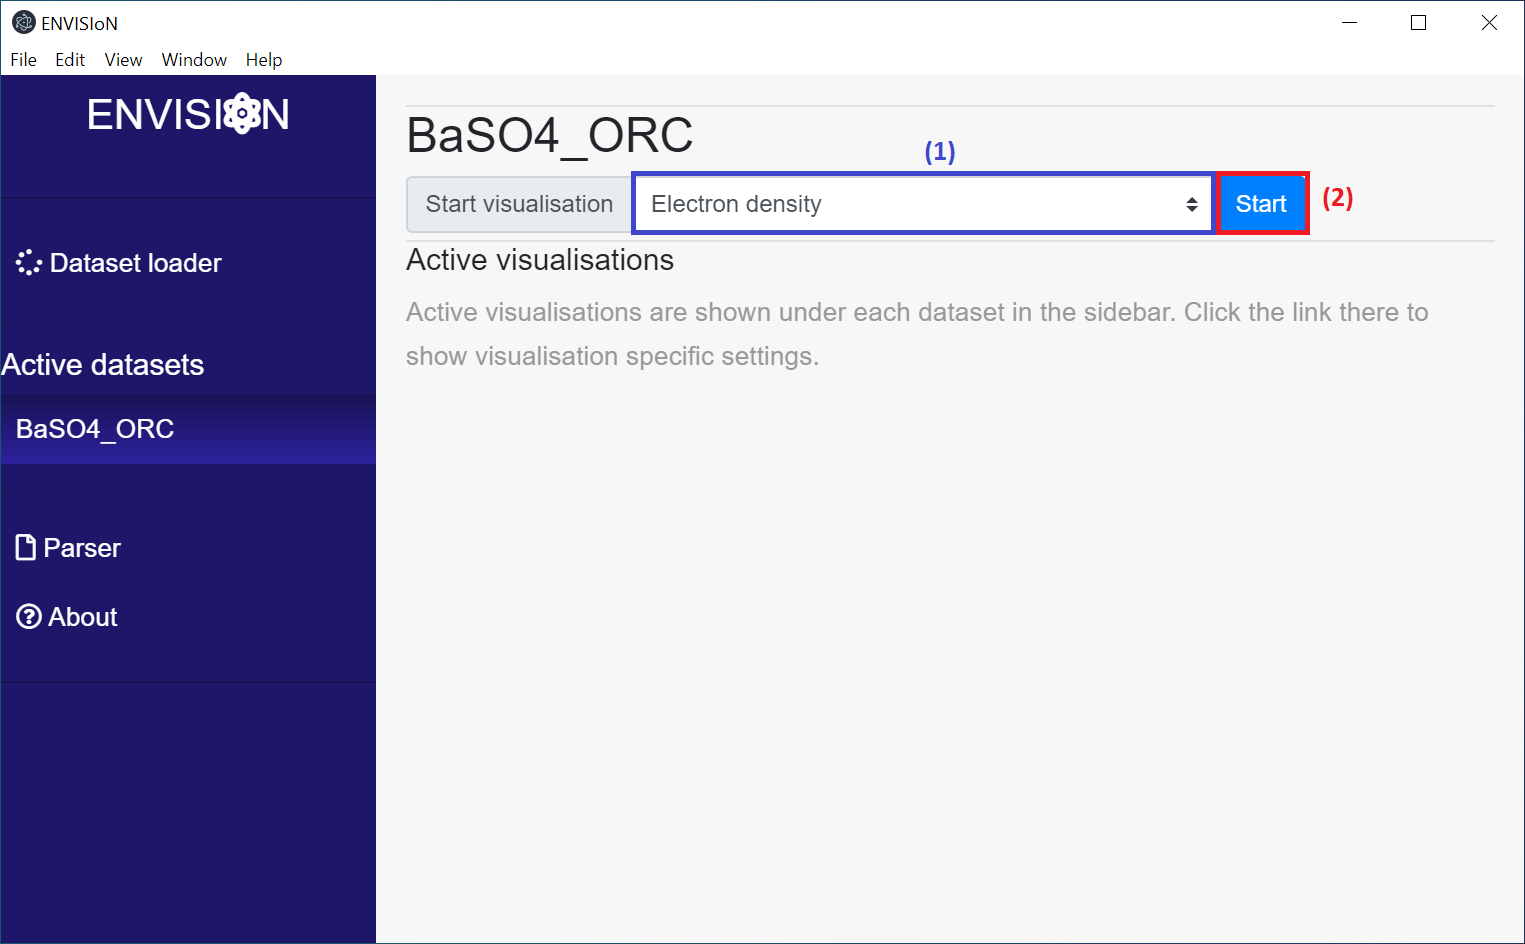
\includegraphics[scale = 0.45]{Images/GUI_Chosevistype.png}
    \caption{Start the visualisation. Here the dataset BaSO4\_ORC is loaded as an example.}
    \label{fig:GUIChosevistype}
\end{figure}

By pressing the area inside the blue box labeled (1) the user can select which visualisation type to visualise from the drop-down menu. The different possible visualisation types are: 

\begin{itemize}
    \item Electron density
    \item Unitcell
    \item Bandstructure 3D
    \item Fermi surface
\end{itemize}

In the red box labeled (2) is the ``Start'' button. When pressing this button the visualisation will start for the chosen visualisation type. The visualisation will appear under the loaded dataset in the sidebar menu. When pressing the visualisation in the sidebar menu new content with visualisation controls will appear to the right. Also the canvas/canvases belonging to the selected visualisation type will pop up next to the GUI.

\subsubsection{Visualisation controls}
When clicking on the ongoing visualisation of a dataset in the sidebar, visualisation controls will appear to the right. These controls are different for different visualisation types. There are only controls for the visualisation types ``Electron density'' and ``Fermi surface''. 

\textbf{Electron density controls}
\newline
If the ongoing visualisation is ``Electron Density'' the controls for interacting with the visualisation are shown in figure \ref{fig:GUICharge} below.

\begin{figure}[H]
    \centering
    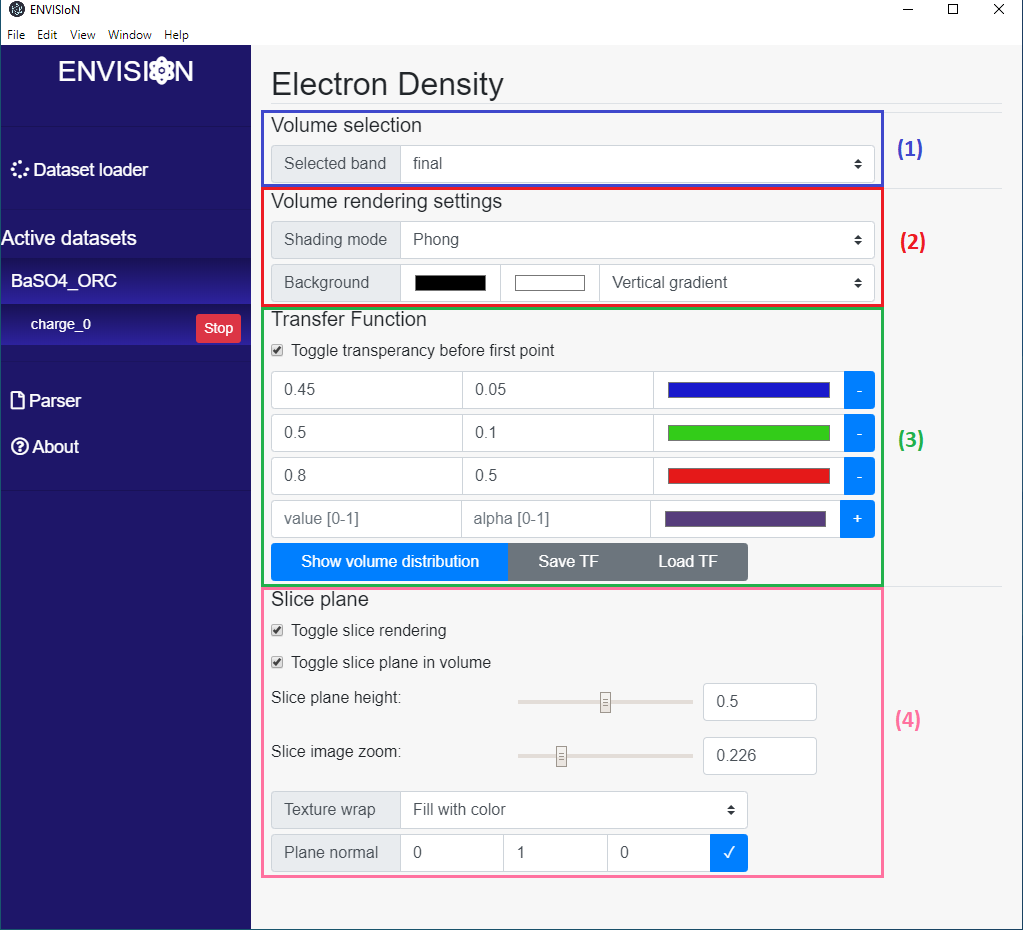
\includegraphics[scale = 0.56]{Images/GUI_Chargecontent.png}
    \caption{The content for the electron density visualisation controls.}
    \label{fig:GUICharge}
\end{figure}

For electron density the user can control the volume selection by selecting band, the volume rendering settings, the transfer function by visualising certain density intervals with different colors and the slice plane to see the electron density in a 2-dimensional plane. In the blue box labeled (1) the user can regulate the volume selection by selecting which band to visualise from a drop-down menu. In the red box labeled (2) the user can select the Shading mode from a drop-down menu and also change the Background color and gradient. In the green box labeled (3) the user can change the transfer function. This is a way to choose different colors for different electron density intervals. The intervals are normalized. The user can also select the blue ``Show volume distribution'' button and then a new diagram will pop up containing information about the volume distribution for the selected dataset. In the pink box labeled (4) the user can configure the slice plan to see a 2-dimensional cross-sectional area of the electron density connected to the 3-dimensional electron density.

\textbf{Fermi surface controls}
\newline
If the ongoing visualisation is ``Fermi surface'' the controls for interacting with the visualisation are shown in figure \ref{fig:GUIFermi} below.

\begin{figure}[H]
    \centering
    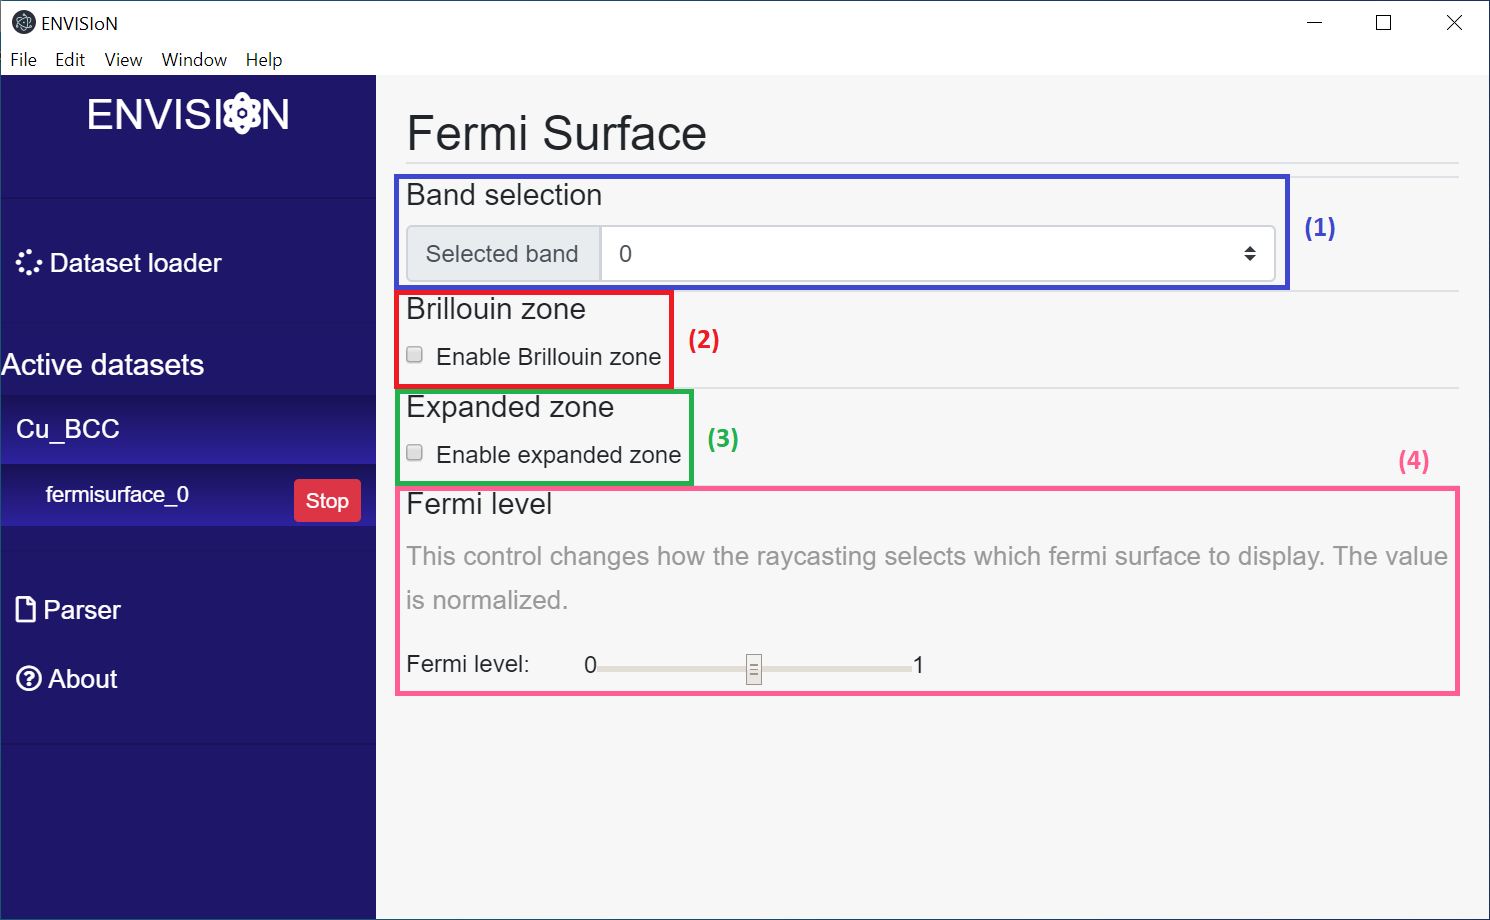
\includegraphics[scale = 0.45]{Images/GUI_Fermicontent.png}
    \caption{The content for the fermi visualisation controls.}
    \label{fig:GUIFermi}
\end{figure}

For fermi surface the user can control which band that should be visualised, enable the Brillouin zone, enable expanded zone and regulate the fermi level. In the blue box labeled (1) the user can select which band to visualise from a drop-down menu. When starting the visualisation the current band will be selected automatically and also the correct fermi level (in the pink box labeled (4)) for each band is set to default. In the red box labeled (2) the user can enable or disable the Brillouin zone by having the checkbox checked or unchecked. In the green box labeled (3) the user can enable or disable expanded zone by having the checkbox checked or unchecked. In the pink box labeled (4) the user can control the fermi level by dragging the slider to the right or to the left. The scale is normalized between 0 and 1.

\subsection{Parser}
If you choose ``Parser'' in the sidebar menu, new content will be exposed to the right, see figure \ref{fig:GUIParser} below. 

\begin{figure}[H]
    \centering
    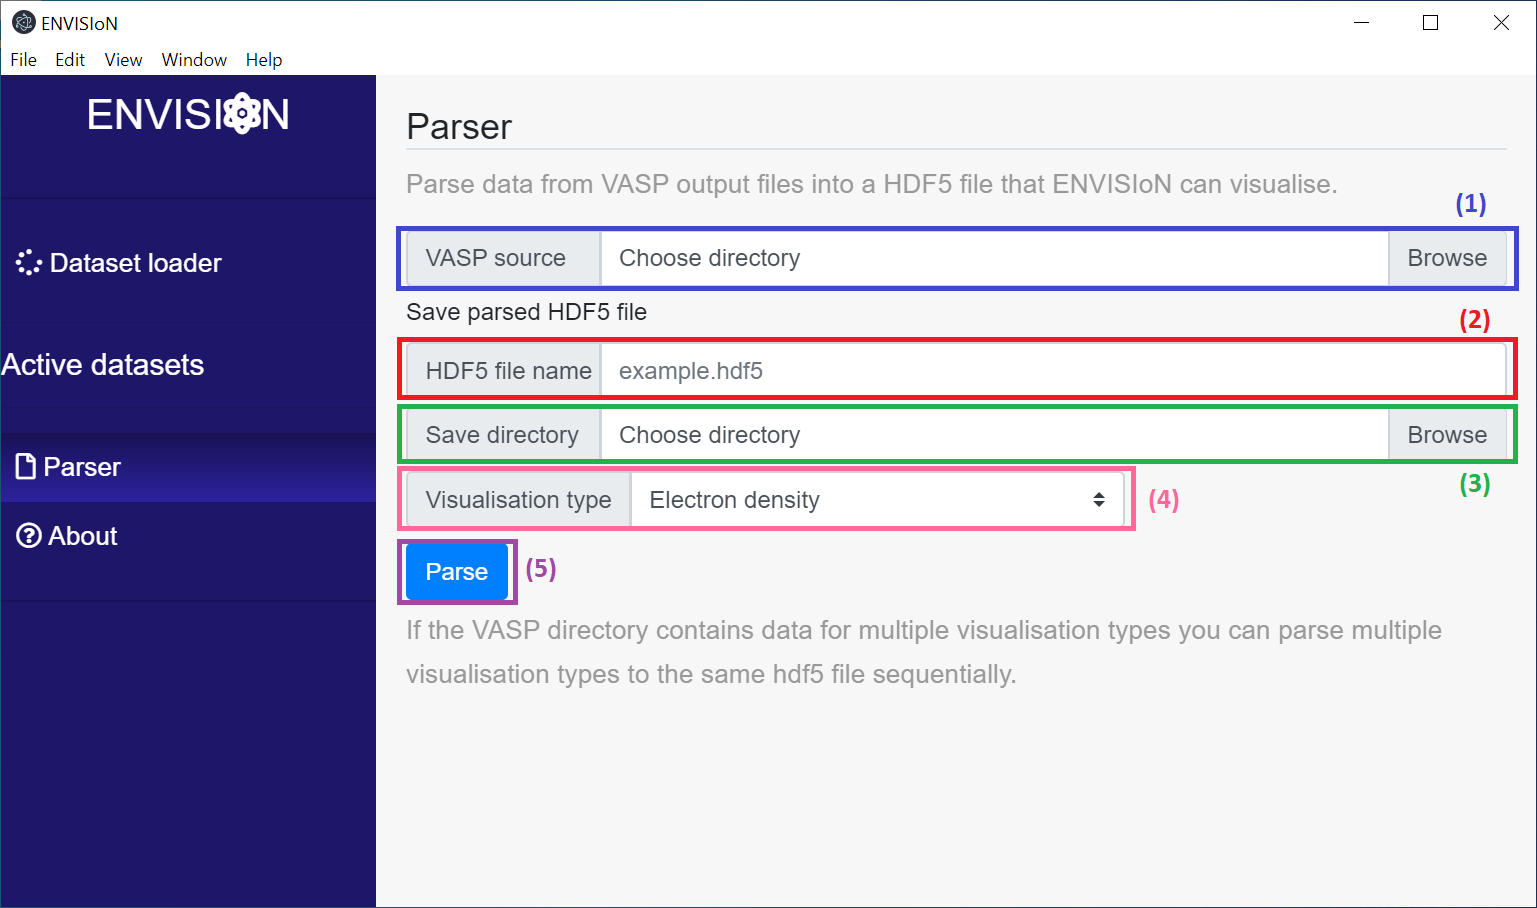
\includegraphics[scale = 0.45]{Images/GUI_Parserstart.png}
    \caption{The content for the parser menu.}
    \label{fig:GUIParser}
\end{figure}

For a quick step-by-step guide, scroll down to section \ref{sec:Parse step-by-step} 

In figure \ref{fig:GUIParser}, in the blue box labeled (1), the path to the directory of VASP files to parse is selected. By clicking on ``Browse'' a new window will appear where the user navigates to the directory of the VASP files on the computer and selects it. In the red box labeled (2) the user writes the name for the new HDF5 file, it needs to end with .hdf5. In the green box labeled (3) the path to the saving directory of the new HDF5 file is selected. When clicking on ``Browse'' a new window will appear where the user navigates to the saving directory and selects it. In the pink box labeled (4) the user can select which visualisation type to parse from a drop-down menu. The possible types to parse are:

\begin{itemize}
    \item Electron density
    \item Bandstructure
    \item Unitcell
    \item Fermi surface
\end{itemize}

In the purple box labeled (5) is the ``Parse'' button. By pressing this button the parser will parse the VASP files and create a HDF5 file in the saving directory. 

\subsubsection{Quick Step-by-step guide}
\label{sec:Parse step-by-step}
Parsing VASP files to a HDF5 file:
\begin{enumerate}
    \item Enter path to VASP directory in (1).
    \item Write name for the HDF5 file in (2).
    \item Enter path to saving directory in (3)
    \item Select type in (4).
    \item Press ``Parse'' in (5).
\end{enumerate}

\subsection{About}
When selecting ``About'' in the sidebar menu there will be new content to the right that contains brief information about ENVISIoN and the project members through the years.

\subsection{If ENVISIoN does not respond or crashes}
If the user have multiple ongoing visualisation or if the user has stopped one visualisation and then want to start another the GUI can stop responding or sometimes even crash. If the GUI falls behind in the number of requests from the user, it will stop responding and a pop up in the GUI will show. The pop up contains the message ``Loading... envision is # requests behind''. See figure \ref{fig:GUINotresponding} below. 

\begin{figure}[H]
    \centering
    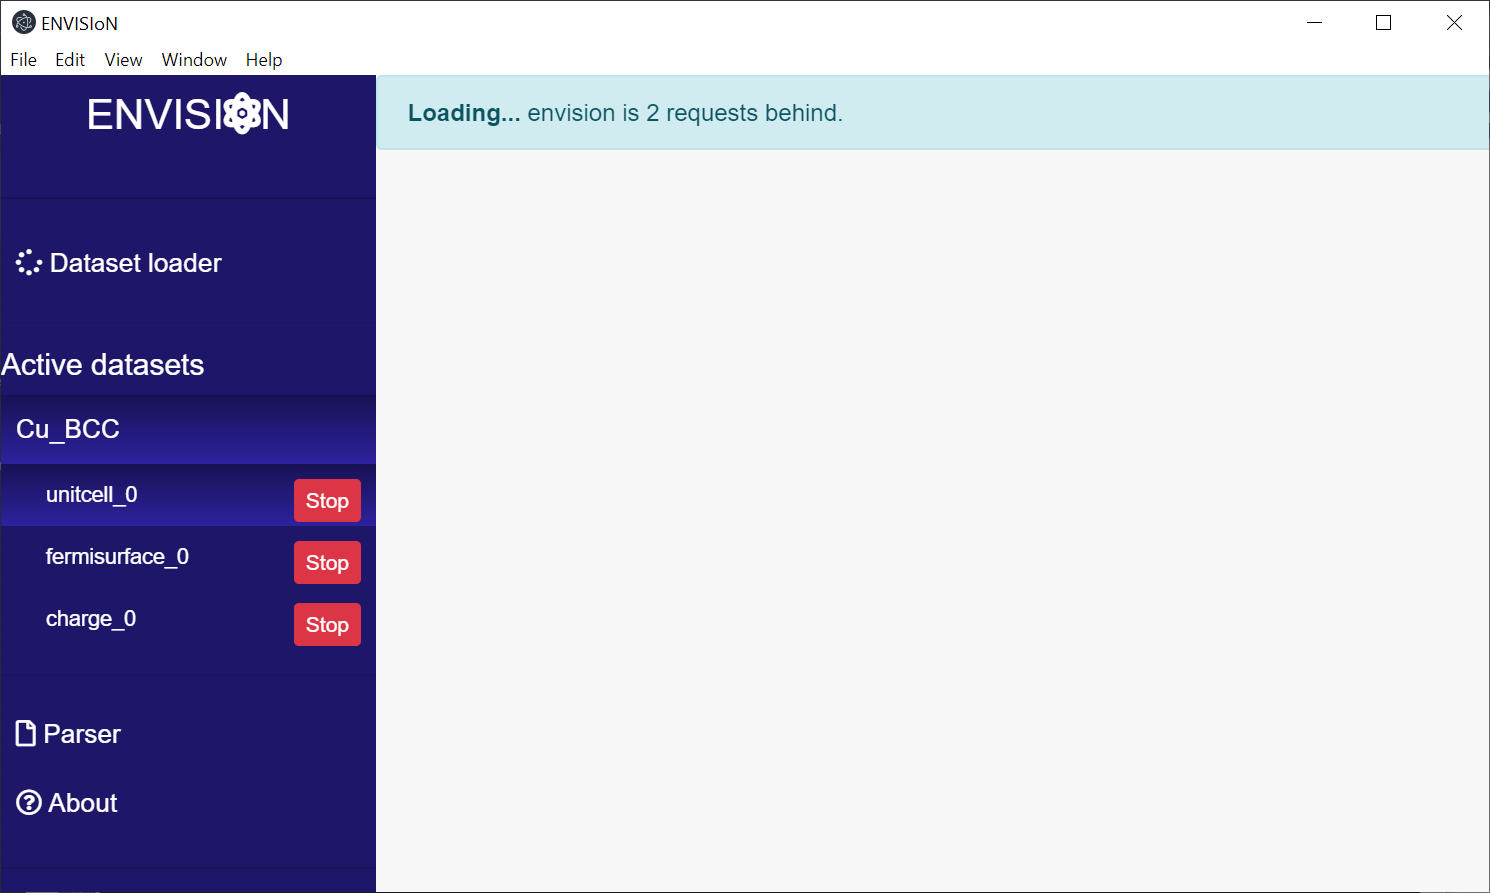
\includegraphics[scale = 0.45]{Images/EnvisionRequestsbehind.png}
    \caption{The pop up when ENVISIoN is a number of requests behind.}
    \label{fig:GUINotresponding}
\end{figure}

To recover from that ENVISIoN is a number of requests behind you can click on ``View'' in the upper menu and then ``Reload'' to reload the GUI. Then you need to start from the beginning and load the dataset once again.

If ENVISIoN is a number of request behind and the user continues to click around in the GUI and tries to load a new dataset or create a new visualisation the GUI will crash. If it does the following message box will pop up, see figure \ref{fig:GUIcrash}.

\begin{figure}[H]
    \centering
    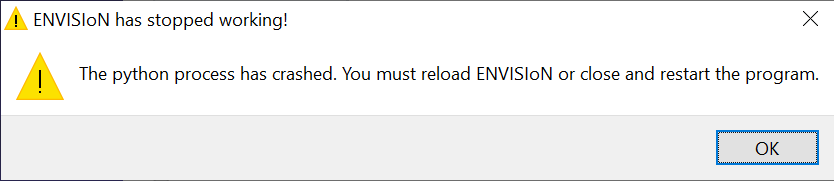
\includegraphics[scale = 0.55]{Images/Envisioncrashed.png}
    \caption{The message box when ENVISIoN crashes.}
    \label{fig:GUIcrash}
\end{figure}

To recover from that ENVISIoN crashes you can either reload the page as mentioned above, or just close the GUI window and restart ENVISIoN.

\newpage
\addcontentsline{toc}{section}{Referenser}
\begin{thebibliography}{99}

\bibitem{API} \textit{API -} URL: \textit{https://www.ne.se/uppslagsverk/encyklopedi/lång/api-(data)} \\ (hämtad 2019-05-16)

\bibitem{BSD2} \textit{BSD2 -} URL: \textit{https://opensource.org/licenses/BSD-2-Clause} \\
(hämtad 2019-05-10)

\bibitem{C++} \textit{C++} URL: \textit{http://www.cplusplus.com/info/description/} (hämtad 2019-01-28).

\bibitem{dict} \textit{Data Structures} URL: \textit{https://docs.python.org/3/tutorial/datastructures.html} (hämtad 2019-05-17).

\bibitem{Fermi-energi} \textit{Solid State Physics -} Neil Ashcroft och David Mermin, 1976, s. 141.

\bibitem{Git} \textit{Git} URL: \textit{https://git-scm.com} (hämtad 2019-01-28).

\bibitem{GUI} \textit{GUI -} URL: \textit{https://www.ne.se/uppslagsverk/encyklopedi/lång/api-(data)}
\\(hämtad 2019-05-10)

\bibitem{High Level Introduction to HDF5} \textit{High Level Introduction to HDF5} URL: \textit{https://support.hdfgroup.org/HDF5/Tutor/HDF5Intro.pdf} (hämtad 2019-02-27).

\bibitem{How To Use HDF5 Files in Python} \textit{How To Use HDF5 Files in Python} URL: \textit{https://www.pythonforthelab.com/blog/how-to-use-hdf5-files-in-python/} (hämtad 2019-02-26).

\bibitem{Inviwo} \textit{Inviwo -} URL: \textit{https://inviwo.org/} (hämtad 2019-05-10)

\bibitem{Python} \textit{Python} URL: \textit{https://www.python.org/} (hämtad 2019-01-28)

\bibitem{Python3} \textit{Python3 -} URL: \textit{https://docs.python.org/3/} (hämtad 2019-05-10)

\bibitem{PyQT} \textit{PyQT -} URL:
\textit{https://www.riverbankcomputing.com/static/Docs/PyQt5/} (hämtad 2019-05-16)

\bibitem{what is array} \textit{Python Arrays} URL: \textit{https://www.programiz.com/python-programming/array\#introduction} (hämtad 2019-05-21).

\bibitem{what is UNIX} \textit{What is UNIX?} URL: \textit{https://www.softwaretestinghelp.com/unix-introduction/} (hämtad 2019-05-21).

\bibitem{wxPython} \textit{wxPython -} URL:
\textit{https://wxpython.org/pages/overview/} (hämtad 2019-05-16)

\bibitem{wxPythonDoc} \textit{wxPython Documentation} URL: \textit{https://docs.wxpython.org/wx.1moduleindex.html} (hämtad 2019-05-17)

\bibitem{Quick Start Guide} \textit{Quick Start Guide} URL: \textit{http://docs.h5py.org/en/stable/quick.html\#appendix-creating-a-file} (hämtad 2019-02-26).

\bibitem{Radial distribution function}
\textit{Radial distribution function} URL: \textit{https://en.wikipedia.org/wiki/Radial\_distribution\_function}
(hämtad 2019-03-03).

\bibitem{HDF group} \textit{The HDF Group, Hierarchical Data Format, version 5 1997-2019} \\
URL: \textit{https://support.hdfgroup.org/HDF5/} 
(hämtad 2018-01-28).

\bibitem{HDF group2}
\textit{The HDF Group. High Level Introduction to HDF5. 23 sept. 2016} \\ URL: \textit{https://support.hdfgroup.org/HDF5/Tutor/HDF5Intro.pdf} (hämtad 2019-01-28).

\bibitem{Unittest} \textit{Unittest} URL: \textit{https://docs.python.org/3/library/unittest.html} (hämtad 2019-03-06).

\bibitem{VASP} \textit{VASP} URL: \textit{https://www.vasp.at/index.php/about-vasp/59-about-vasp} (hämtad 2019-02-26).




 
\end{thebibliography}
\newpage
\appendix
\newpage
\section{Appendix A - ENVISIoNs HDF5-filstruktur} \label{sec:appendixHDF5}
\begin{figure}[H]
  \centering
 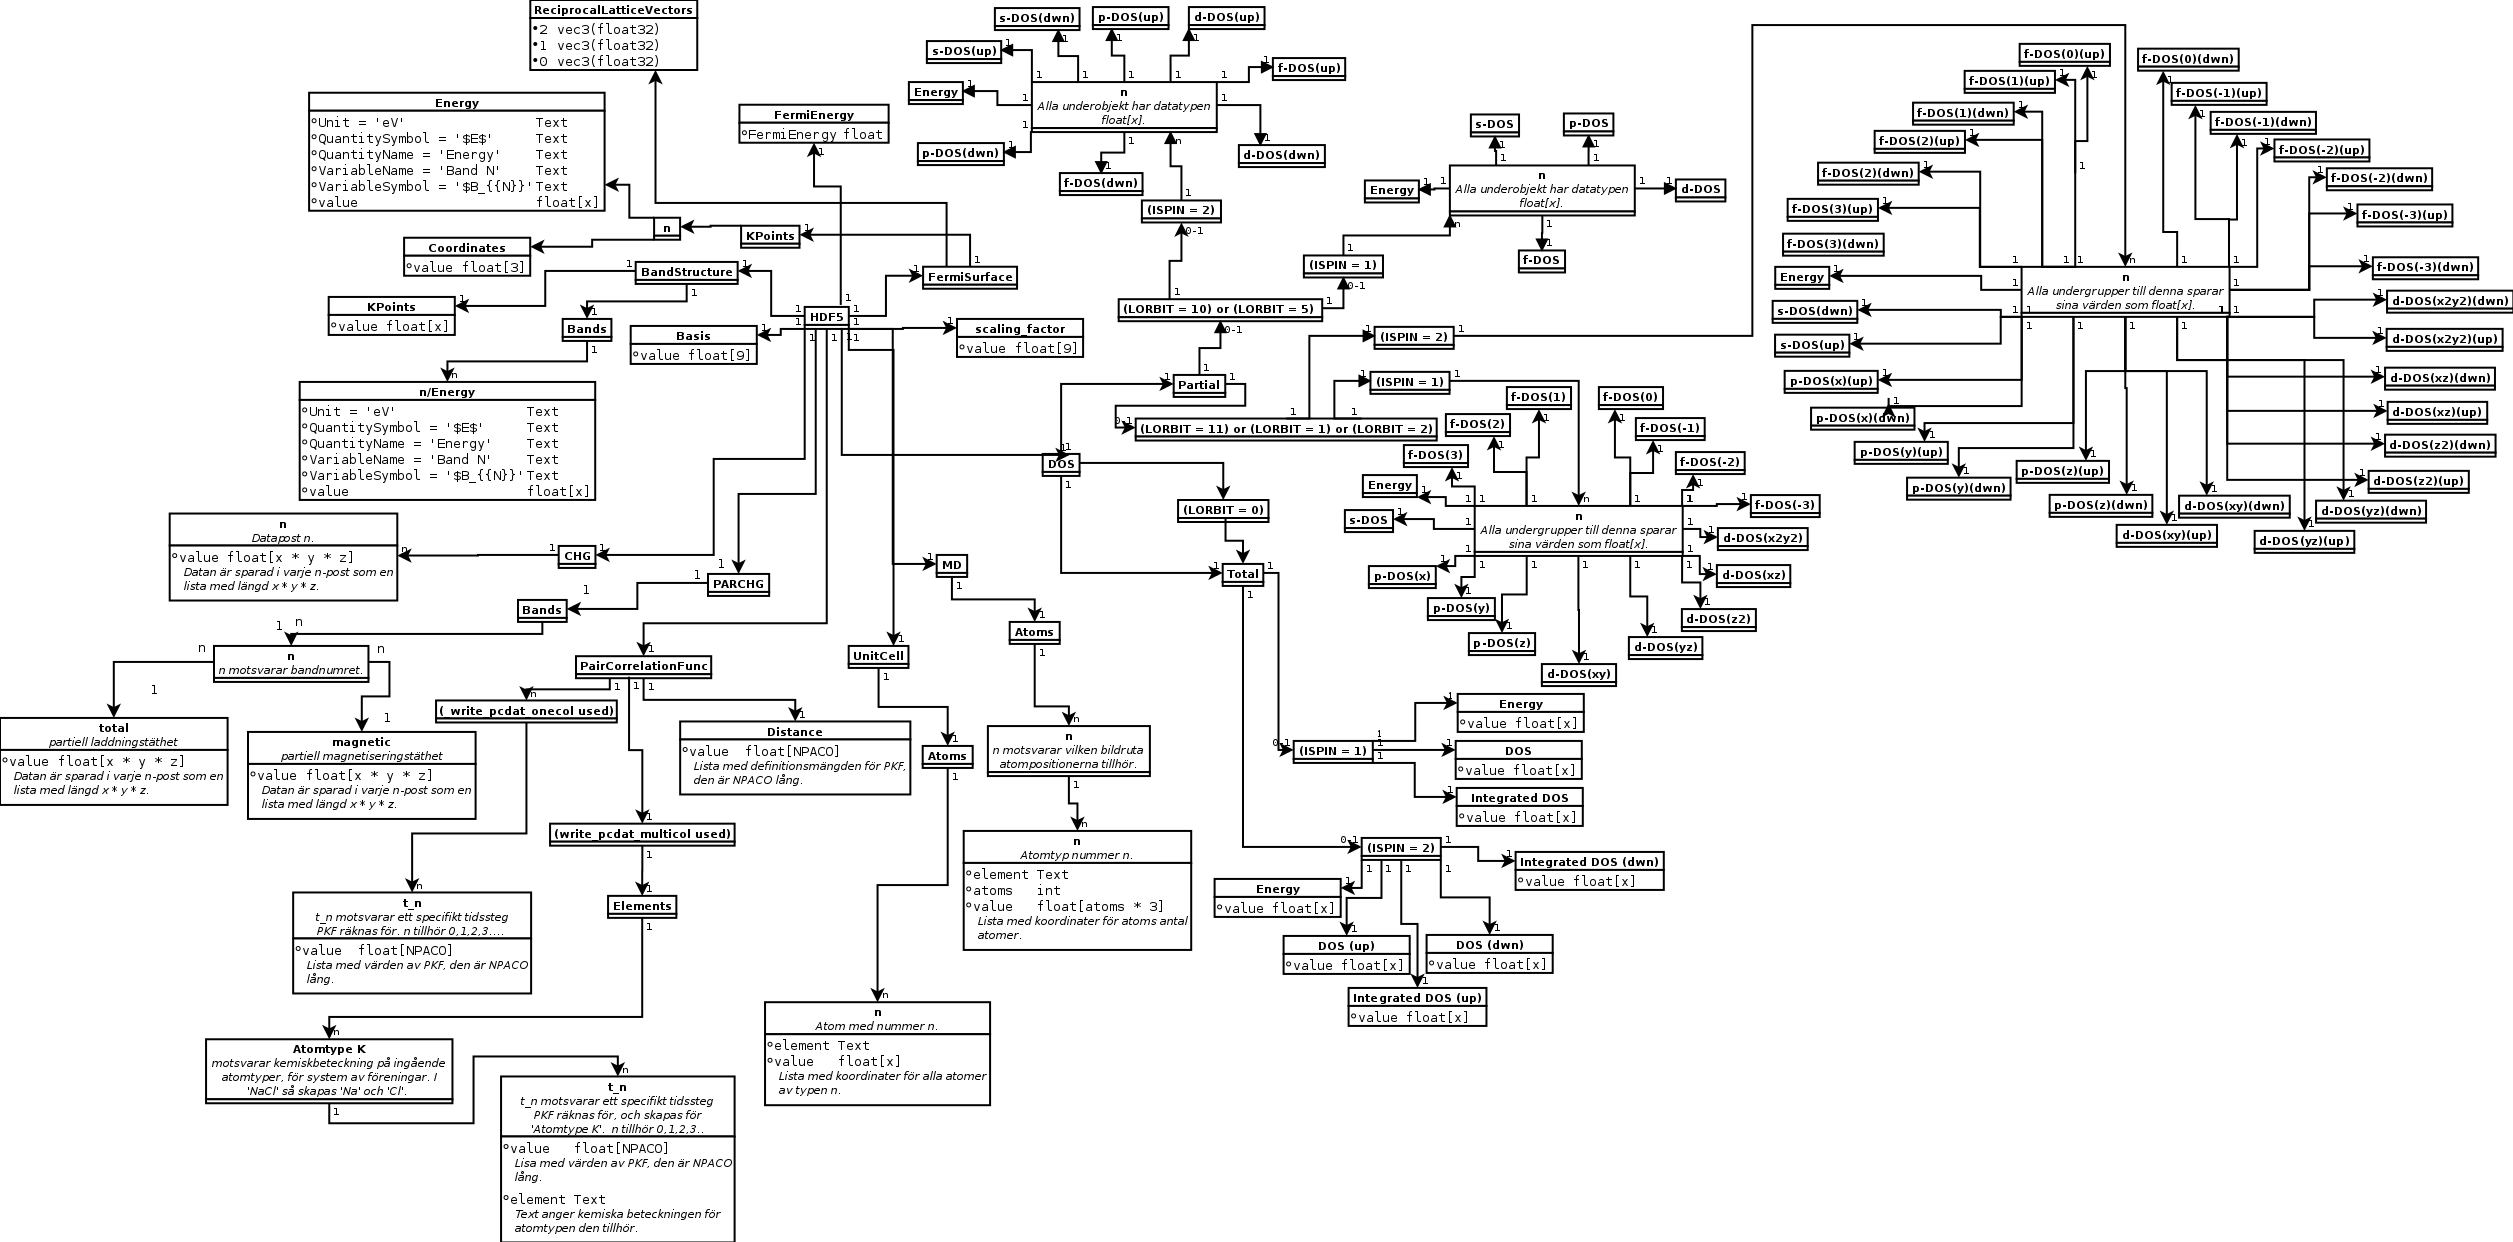
\includegraphics[angle=270,scale=0.26]{images/UPDATE-hdf5-dataformat3modi.png}
  %\caption{En bild över HDF5-filformat som används i ENVISIoN.}
  %\label{fig:ENVISIoNsHDF5_appendix}
\end{figure}
\newpage

\newpage 
\newpage
\section{Appendix B - Sökvägar till filer relevanta för GUI:t} \label{sec:GUIAppendix}
 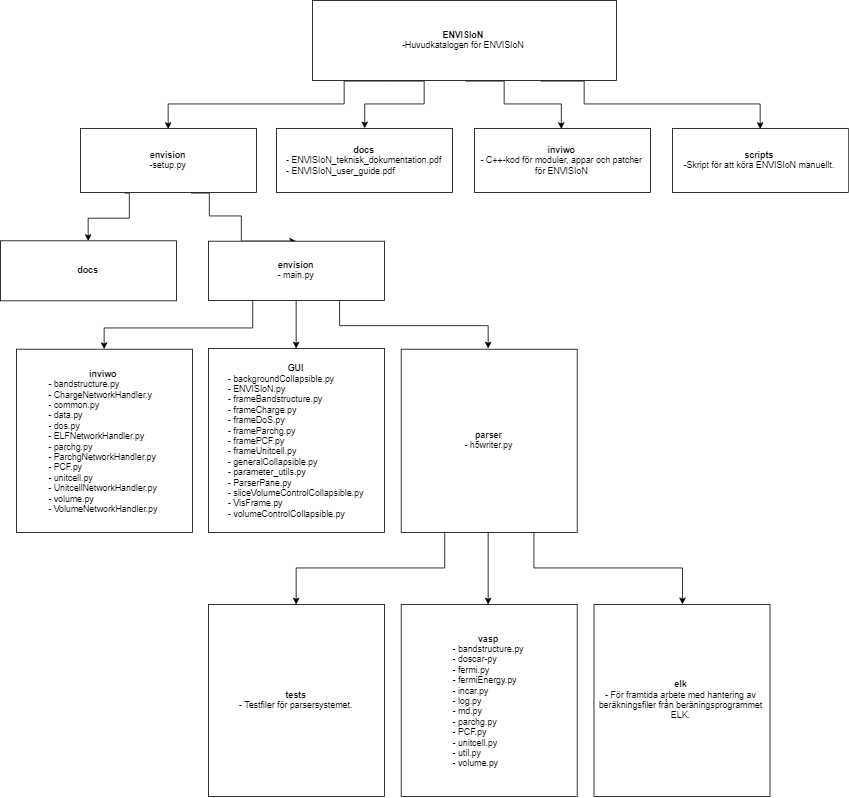
\includegraphics[angle=270,scale=0.6]{images/DirTree.png}

\newpage 
\section{Licens}
\label{ref:licens}
Copyright (c) 2017: Josef Adamsson, Robert Cranston, David Hartman, Denise Härnström, Fredrik Segerhammar. \textit{(Teknisk dokumentation - release 1)}\newline
Copyright (c) 2018: Anders Rehult, Andreas Kempe, Marian Brännvall, Viktor Bernholtz. \textit{(Teknisk dokumentation - release 2)}\newline
Copyright (c) 2019: Linda Le, Abdullatif Ismail, Anton Hjert, Lloyd Kizito and Jesper Ericsson. \textit{(Teknisk dokumentation - release 3)}\newline
Copyright (c) 2017: 2019 - Rickard Armiento, Johan Jönsson

All rights reserved.

Redistribution and use in source and binary forms, with or without
modification, are permitted provided that the following conditions are met:

1. Redistributions of source code must retain the above copyright notice, this list of conditions and the following disclaimer.\newline
2. Redistributions in binary form must reproduce the above copyright notice, this list of conditions and the following disclaimer in the documentation and/or other materials provided with the distribution.

THIS SOFTWARE IS PROVIDED BY THE COPYRIGHT HOLDERS AND CONTRIBUTORS AS IS AND ANY EXPRESS OR IMPLIED WARRANTIES, INCLUDING,
BUT NOT LIMITED TO, THE IMPLIED WARRANTIES OF MERCHANTABILITY AND FITNESS FOR A PARTICULAR PURPOSE ARE DISCLAIMED. IN NO EVENT
SHALL THE COPYRIGHT OWNER OR CONTRIBUTORS BE LIABLE FOR ANY DIRECT, INDIRECT, INCIDENTAL, SPECIAL, EXEMPLARY, OR CONSEQUENTIAL
DAMAGES (INCLUDING, BUT NOT LIMITED TO, PROCUREMENT OF SUBSTITUTE GOODS OR SERVICES; LOSS OF USE, DATA, OR PROFITS; OR BUSINESS
INTERRUPTION) HOWEVER CAUSED AND ON ANY THEORY OF LIABILITY, WHETHER IN CONTRACT, STRICT LIABILITY, OR TORT (INCLUDING
NEGLIGENCE OR OTHERWISE) ARISING IN ANY WAY OUT OF THE USE OF THIS SOFTWARE, EVEN IF ADVISED OF THE POSSIBILITY OF SUCH DAMAGE.

\newpage 
\section{Dokumentets proveniens}
\label{sec:provenance}

\begin{itemize}
\item 2019: Teknisk dokumentation - release 3: skrevs av: Linda Le, Abdullatif Ismail, Anton Hjert, Lloyd Kizito and Jesper Ericsson.
\item 2018: Teknisk dokumentation - release 2: skrevs av: Anders Rehult, Andreas Kempe, Marian Brännvall, Viktor Bernholtz.
\item 2017: Teknisk dokumentation - release 1: skrevs av: Josef Adamsson, Robert Cranston, David Hartman, Denise Härnström, Fredrik Segerhammar.
\item Vissa ändringar har genom åren införts av: Rickard Armiento, Johan Jönsson
\end{itemize}

\end{document}
